\documentclass{beamer} %[hyperref={pdfpagelabels=false}]
\usepackage{beamerthemeFreiburg_beamer}
\usepackage{lmodern}

\PassOptionsToPackage{dvipsnames}{xcolor}  % needed to get colors working in certain environments
\usepackage[utf8]{inputenc}
\usepackage[T1]{fontenc}
\usepackage[german]{babel}
\usepackage{graphicx}
\usepackage{wrapfig}  % used for wrapping a figure alternative to using minipages
\usepackage{amsmath}
\usepackage{amsfonts}
\usepackage{amssymb}
%\usepackage[hidelinks]{hyperref}  % removes coloring for links
\usepackage{cleveref}
\usepackage{tikz}
\usepackage{tikz-cd}
\usepackage{nicefrac}  % adds \nicefrac alternative to regular \frac
\usepackage{mathtools}
\usepackage{enumerate}
\usepackage{cancel}  % adds \cancel which adds strikethrough
%\usepackage{tocloft}
\usepackage{tcolorbox}
\usepackage{bm}  % adds \bm to make symbols bold, replaces outdated \boldsymbol
%\usepackage[shortlabels]{enumitem}
%\usepackage{placeins}
\usepackage{booktabs}
\usepackage{wasysym}

\graphicspath{ {Bilder/} }

%\usepackage[margin=1in]{geometry}  % changes the margins on all pages
\usepackage{url}
\usepackage{subcaption}
\usepackage[tablewithin=section]{caption}

%SI-unix
%\usepackage{array}
\usepackage[per=slash,
decimalsymbol=comma,
loctolang={DE:ngerman,UK:english},
]{siunitx}	
\sisetup{locale = DE}

%\usetikzlibrary{calc}
%\usetikzlibrary{decorations.pathmorphing,patterns}
%\usetikzlibrary{arrows}
%\usetikzlibrary{decorations.pathreplacing}

%\usetikzlibrary{snakes}

% Andrez:
%\usepackage{epigraph}  % adds \epigraph used to add fancy quotes to the beginning of chapters
%\usepackage{fancyhdr}
%\setlength{\parskip}{1em}
%\setlength{\headheight}{35pt}
%\setlength\epigraphwidth{.8\textwidth}
% alt math font
%\usepackage{eulervm}  % switches to alternate math font, usually requires extra download


%Environments und Newcommands:


% general commands

% zu zeigen symbol
\newcommand{\zz}{\fontfamily{cmss} \selectfont{Z\kern-.61em\raise-0.7ex\hbox{Z}:}}
% build over
\newcommand{\bov}[2]{\buildrel{#2} \over{#1}}
% better looking := (defined as)
\newcommand*{\defeq}{\mathrel{\vcenter{\baselineskip0.5ex \lineskiplimit0pt \hbox{\scriptsize.}\hbox{\scriptsize.}}}=}
\newcommand*{\eqdef}{=\mathrel{\vcenter{\baselineskip0.5ex \lineskiplimit0pt \hbox{\scriptsize.}\hbox{\scriptsize.}}}}

% integral differential d
\newcommand{\dif}{\mathop{}\!\mathrm{d}}
\newcommand{\difi}[1]{\mathrm{d}#1\mathop{}\!}

\newcommand{\prt}[2]{\frac{\partial #1}{\partial #2}}  % used for partial derivatives, tip: input #1 can be left blank
\newcommand{\prd}[2]{\frac{\tx{d} #1}{\tx{d} #2}}  % used for absolute (standart) derivatives, tip: input #1 can be left blank

\newcommand{\dd}{\tx{d}}


%Mathe:
\newcommand{\verteq}{\rotatebox{90}{$\,=$}}  % used for commands below
\newcommand{\equalto}[2]{\underset{\scriptstyle\overset{\mkern4mu\verteq}{#2}}{#1}}  % adds equal to underneath
\newcommand{\equaltoup}[2]{\overset{\scriptstyle\underset{\mkern4mu\verteq}{#2}}{#1}}  % adds equal to above
\newcommand{\custo}[3]{\underset{\scriptstyle\overset{\mkern4mu\rotatebox{-90}{$\,#1$}}{#3}}{#2}}  % same as above but replaces equal sign with input #1
\newcommand{\custoup}[3]{\overset{\scriptstyle\underset{\mkern4mu\rotatebox{-90}{$\hspace{-3pt} #1$}}{#3}}{#2}}
\newcommand{\casess}[4]{\left\{ \begin{array}{ll} {#1} & {#2} \\ {#3} & {#4} \end{array} \right.}  % used to indicate to the reader that something is missing here


%Text:
\newcommand{\tx}[1]{\textrm{#1}}
\newcommand{\const}{\tx{const.}}

\newcommand{\ul}[1]{\underline{#1}}
\newcommand{\ol}[1]{\overline{#1}}
\newcommand{\ub}[1]{\underbrace{#1}}
\newcommand{\ob}[1]{\overbrace{#1}}

\newcommand{\hfw}{\color{RubineRed}\tx{ $\star$hier fehlt was$\star$ } \color{black}}  % used to indicate to the reader that something is missing here 


%Spezielles:


%Theo:
\newcommand{\lag}{\mathcal{L}}  % used for Lagrange function
\newcommand{\ham}{\mathcal{H}}  % used for Hamiltonian function
\newcommand{\gre}{\mathcal{G}}  % used for Green's function
\newcommand{\eofr}{\vec{E}(\vec{r})}
\newcommand{\pofr}{\Phi(\vec{r})}
\newcommand{\grr}{\mathcal G(\vec{r},\vec{r}')}
\newcommand{\vphi}{\varphi}
\newcommand{\vabla}{\vec{\nabla}}


%LA:
\newenvironment{bew}[1]{\subsection{Bew: #1}}{\hfill$\square$}
\newcommand{\Bew}[2]{\begin{bew}{#1}#2\end{bew}}
\newcommand{\enph}{F: V \to V \textrm{ Endomorphismus}}

\newcommand{\im}{\tx{im}}
\newcommand{\spa}{\tx{span}}
\newcommand{\adj}{\tx{adj}}
\newcommand{\grad}{\tx{grad}}
\newcommand{\ord}{\tx{ord}}

\newcommand{\basis}[3]{\{#1_{#2}, \dots, #1_{#3}\}}
\newcommand{\ska}[2]{\langle #1 , #2 \rangle}  % scalar product of input 1, and 2 can also be used for braket notation
\newcommand{\dmat}[3]{\begin{pmatrix} #1_{#2}&&\\ &\ddots& \\ && #1_{#3} \end{pmatrix}}


%Ex:
\newcommand{\kq}{\frac{1}{4\pi\epsilon_0}}  % writes out the whole constant k from electrostatic
\newcommand{\kqq}{\frac{\mu_0}{4\pi}}  % writes out the constant from magnetostatic
\newcommand{\uind}{U_{\tx{ind}}}
\newcommand{\folie}[1]{\color{gray}[Folie: #1]\color{black}}  % used to tell the reader that there was multimedia content during a lecture
\newcommand{\versuch}[1]{\color{red!50!black} \textbf{Versuch:} \color{black} \textbf{#1}\\ }  % used to tell the reader that there was a live experiment

\newcommand{\mau}{$\buildrel \mathcal{O} \over{\textbf{.}}$}  % the extreme Waldmann exclamation mark recreated in latex by Markus


% Lab commands:
\newcommand\mean{\begin{equation}
	\frac{\sum_{i=1}^n x_i}{n}\label{mean}
	\end{equation}}  % shortcut for the standard Mean function

\newcommand\meanstd{\begin{equation}
	s_x=\sqrt{\frac{1}{n-1}\sum_{i=1}^n(x_i-\overline{x})^2}\label{meanstd}
	\end{equation}}  % shortcut for the standard derivative mean function

\newcommand\prodquo{\begin{equation}\left\vert\frac{\Delta z}{z}\right\vert=\sqrt{\left(a\frac{\Delta x}{x}\right)^2+\left(b\frac{\Delta y}{y}\right)^2+\ldots}\textrm{ f\"ur }z=x^a\ y^b\ldots\end{equation}}

\newcommand\tfuncd{\begin{equation}
	t=\frac{\vert x_n-y_n\vert}{\sqrt{x_s^2+y_s^2}}
	\end{equation}}

\newcommand\tfunc{\begin{equation}
	t=\frac{\vert x-y_0\vert}{u_x}
	\end{equation}}


% ANDREZ
\newcommand{\summ}[2]{\sum_{#1}^{#2}}
\newcommand{\intt}[2]{\int_{#1}^{#2}}
\newcommand{\lcom}[1]{\color{MidnightBlue}#1\color{black}}  % used to indicate to the reader that this content was transcribed from the lecture
\newcommand{\bei}{\emph{Beispiel: }}
\newcommand{\bem}{\emph{Bemerkung:}}


% Boxen:

\tcbuselibrary{theorems}

% mahlt eine box nur um den text mit titel
\newtcbox{\fribox}[1]{nobeforeafter,colback=white,colframe=red!75!black,fonttitle=\bfseries,title=#1,sharp corners,tcbox raise base}

% mahlt eine große box um alles mit titel
\newcommand{\frbox}[2]{\begin{tcolorbox}[colback=white,colframe=red!75!black,fonttitle=\bfseries,title=#1]#2\end{tcolorbox}}

% mahlt eine box nur um den text
\newtcbox{\ribox}{nobeforeafter,colback=white,colframe=red!75!black,sharp corners,tcbox raise base}

% mahlt eine große box um alles was drinnen ist
\newcommand{\rbox}[1]{\begin{tcolorbox}[colback=white,colframe=red!75!black]#1\end{tcolorbox}}

% mahlt eine box um mathe innerhalb mathmode
\newcommand{\rmbox}[1]{\tcboxmath[colback=white,colframe=red!75!black]{#1}}

% super box (looks like regular boxed but wraps around anything)
\newenvironment{supbox}{\begin{tcolorbox}[colback=white,colframe=black,sharp corners,boxrule=.5pt]}{\end{tcolorbox}}

% the Big Black Box, can be used to separate examples or review material from the main text (used for Wiederholung)
\newcommand{\bbb}[2]{\begin{tcolorbox}[colback=white,colframe=black,fonttitle=\bfseries,title=#1,sharp corners,tcbox raise base]#2\end{tcolorbox}}

% array type box with title
\newenvironment{zebox}[1]{\begin{array}{|c|}
		\multicolumn{1}{l}{\tx{#1}} \\
		\hline
		\displaystyle
	}{\\ \hline
\end{array}}

% arrow list
%\newlist{arrowlist}{itemize}{1}
%\setlist[arrowlist]{label=$\Rightarrow$}


% optional:

\renewcommand{\vec}[1]{\bm{#1}}

% changed because of preferred looks
\renewcommand{\epsilon}{\varepsilon}
%\renewcommand{\paragraph}[1]{\subsubsection{#1}}  % changed oddly behaving paragraphs to simple subsubsections which are not numbered nor in the toc

% nur in Theo benutzt !!!
% \renewcommand{\Phi}{\varPhi}

% evtl:
% \renewcommand{\boxed}{\rmbox}


% Tikz definitions:

\def\centerarc[#1](#2)(#3:#4:#5)% Syntax: [draw options] (center) (initial angle:final angle:radius)
{ \draw[#1] ($(#2)+({#5*cos(#3)},{#5*sin(#3)})$) arc (#3:#4:#5); }

\def\checkmark{\tikz\fill[scale=0.4](0,.35) -- (.25,0) -- (1,.7) -- (.25,.15) -- cycle;}  % checkmark used for proofs

\tikzset{
	annotated cuboid/.pic={
		\tikzset{%
			every edge quotes/.append style={midway, auto},
			/cuboid/.cd,
			#1
		}
		\draw [every edge/.append style={pic actions, densely dashed, opacity=.5}, pic actions]
		(0,0,0) coordinate (o) -- ++(-\cubescale*\cubex,0,0) coordinate (a) -- ++(0,-\cubescale*\cubey,0) coordinate (b) edge coordinate [pos=1] (g) ++(0,0,-\cubescale*\cubez)  -- ++(\cubescale*\cubex,0,0) coordinate (c) -- cycle
		(o) -- ++(0,0,-\cubescale*\cubez) coordinate (d) -- ++(0,-\cubescale*\cubey,0) coordinate (e) edge (g) -- (c) -- cycle
		(o) -- (a) -- ++(0,0,-\cubescale*\cubez) coordinate (f) edge (g) -- (d) -- cycle;
		\path [every edge/.append style={pic actions, |-|}]
		%(b) +(0,-5pt) coordinate (b1) edge ["\cubex \cubeunits"'] (b1 -| c)
		%(b) +(-5pt,0) coordinate (b2) edge ["\cubey \cubeunits"] (b2 |- a)
		%(c) +(3.5pt,-3.5pt) coordinate (c2) edge ["\cubez \cubeunits"'] ([xshift=3.5pt,yshift=-3.5pt]e)
		;
	},
	/cuboid/.search also={/tikz},
	/cuboid/.cd,
	width/.store in=\cubex,
	height/.store in=\cubey,
	depth/.store in=\cubez,
	units/.store in=\cubeunits,
	scale/.store in=\cubescale,
	width=10,
	height=10,
	depth=10,
	units=cm,
	scale=.1,
}



% other settings
\hbadness=99999  % removes unnecessary hbadness warnings

\title[Emulsionen ]{Emulsionen}
% \\ \ \\ \ \\  1.Grundlagen  \\ \ \\  2.Emulgatoren \\ \ \\ 3.Erstellen von Emulsionen  \\ \ 
\subtitle[Seminar Physik in der Küche]{}
\date[15. Januar 2020]{15. Januar 2020}
\author[Markus, Phillip und Kim]{Ye Joon Kim, Markus \"Osterle, Philipp Bronner}
\logo{
\includegraphics[scale=0.25]{image.jpeg}}
%\logo{\includegraphics[scale=0.08]{ap,550x550,12x12,1,transparent,t.png}}
%\logo{\includegraphics[scale=0.1]{Aperture_Science_grey.png}}
%\logo{\includegraphics[scale=0.18]{Aperture_Science_yellow_monitor.png}}

\begin{document}
\begin{frame}
\titlepage
\end{frame}

\section{Grundlagen}

\begin{frame}
\frametitle{Grundlagen zu Emulsionen}
\begin{itemize}
	\item IUPAC Definition: "\textit{Fluid system in which liquid droplets are dispersed in a liquid.}"\pause
	\item In der Küche nur Wasser-Öl und Öl-Wasser Emulsionen
\end{itemize}
	\begin{figure}
		\centering
		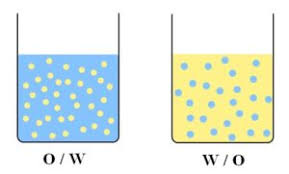
\includegraphics[width=0.5\linewidth]{owwo.jpg}
		\caption{Öl-Wasser und Wasser-Öl Emulsionen}
	\end{figure}
\begin{itemize}
	\item{Wichtige Terme:Disperse/Kontinuierliche Phasen, Interface}
\end{itemize}
\end{frame}

\subsection{Polarität}

\begin{frame}
\frametitle{Polarität von Wasser und Lösbarkeit}
\begin{itemize}
	\item Wasser ist polar, Öl (Fett) ist nicht polar
\end{itemize}
\begin{minipage}[h]{0.49\textwidth}
	\begin{figure}[h]
		\centering
		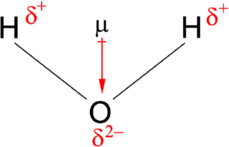
\includegraphics[width=0.8\linewidth]{water.png}
	\end{figure}
\end{minipage}
\begin{minipage}[h]{0.49\textwidth}
	\begin{figure}[h]
		\centering
		
\includegraphics[width=\linewidth]{fett.png}
	\end{figure}
\end{minipage}
\begin{itemize}
	\item $\Rightarrow$ Polare Moleküle in Wasser und Nichtpolare Moleküle in Fett löslich. 
\end{itemize}
\end{frame}

\subsection{Grenzflächen}

\begin{frame}
\frametitle{Verhalten von Flüssig-Flüssig Grenzflächen und Oberflächenspannung}
\begin{figure}
	\centering
	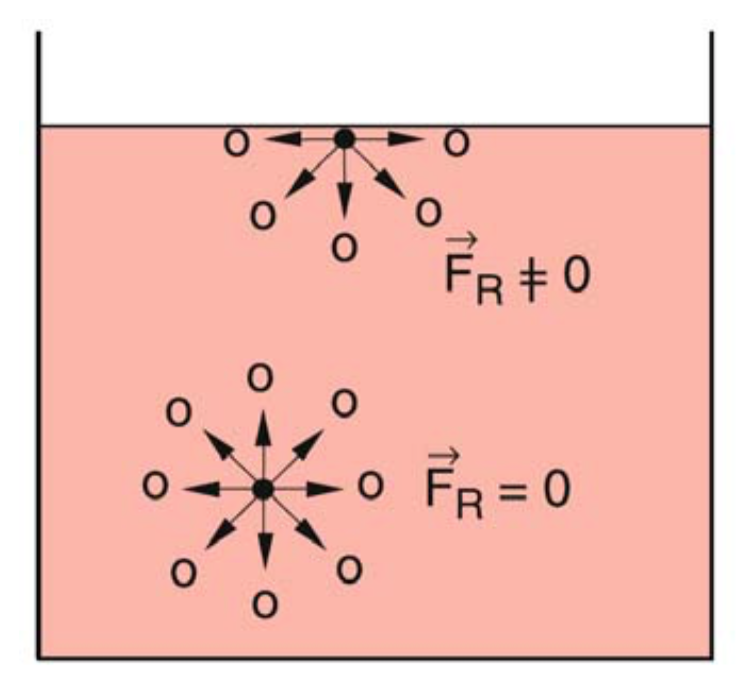
\includegraphics[width=0.3\linewidth]{of.png}
\end{figure}

\begin{itemize}
	\item{Energie wird benötigt, um zusätzliche Oberfläche zu bilden}
\end{itemize}

\begin{equation}
\Delta W = \sigma_0\cdot \Delta A
\end{equation}
\pause
\begin{itemize}
	\item $\Rightarrow$ Es bilden Kugelförmige Tröpfchen
\end{itemize}
\end{frame}
\begin{frame}
	\frametitle{Arten von Emulsion-Instabilitäten}
\begin{figure}
	\centering
	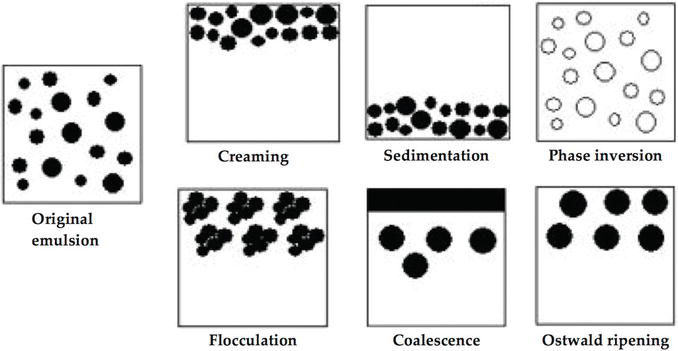
\includegraphics[width=\linewidth]{F1.png}
\end{figure}
\end{frame}

\begin{frame}{Instabilität von Emulsionen}
	\begin{itemize}
		\item Instabilität von Emulsionen kann gemessen werden.
	\end{itemize}
\begin{equation}
\textrm{Emulsion Stability}=\frac{V_B-V_A}{V_B}
\end{equation}
\begin{itemize}
	\item $\Rightarrow$ Unterscheidung in Kurz- und Langzeitstabilität
\end{itemize}
\end{frame}
%Markus:

\section{Emulsionen Herstellen}

\begin{frame}{Herstellung von Emulsionen}
	\begin{block}{}
		\begin{itemize}
			\item Vorvermischen der Komponenten zu einer grobdispersen \textbf{Rohemulsion}\pause
			\item Deformieren und \textbf{Aufbrechen} von Tropfen\pause
			\item \textbf{Stabilisieren} der neu geschaffenen Grenzfläche
		\end{itemize}
	\end{block}
\end{frame}

\subsection{Tropfenaufbruch}

\begin{frame}{Mechanismen zum Tropfenaufbruch}
	\begin{minipage}{0.6\linewidth}
		Laplacedruck:
		\begin{equation*}
		p_L = \gamma \left(\frac{1}{R_1} + \frac{1}{R_2}\right)
		\end{equation*}
		Kugelförmige Tropfen:
		\begin{equation*}
		p_L = \gamma \left(\frac{4}{D}\right)
		\end{equation*}
		Weberzahl
		\begin{equation*}
		We = \frac{\sigma}{p_L}
		\end{equation*}
	\end{minipage}%
	\begin{minipage}{0.4\linewidth}
		\flushright
		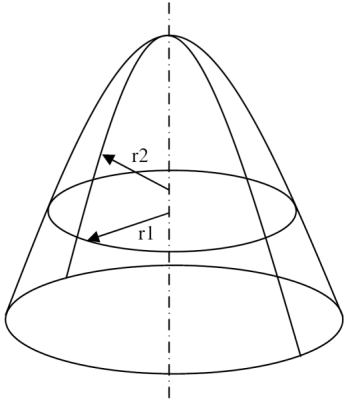
\includegraphics[width=0.8\linewidth]{Markus/Synklastisch}\\
		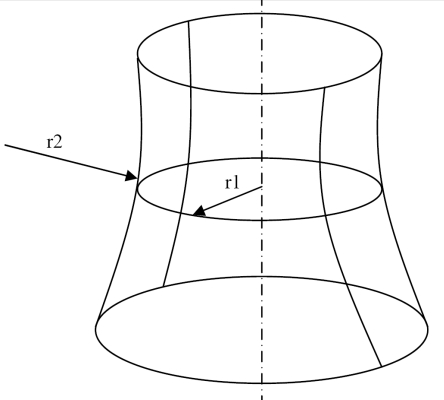
\includegraphics[width=\linewidth]{Markus/Antiklastisch}
	\end{minipage}
\end{frame}

\begin{frame}{Laminare Strömung}
	\begin{itemize}
		\item Rotationsströmung
		\item Scherströmung
		\item Dehnströmung
	\end{itemize}
	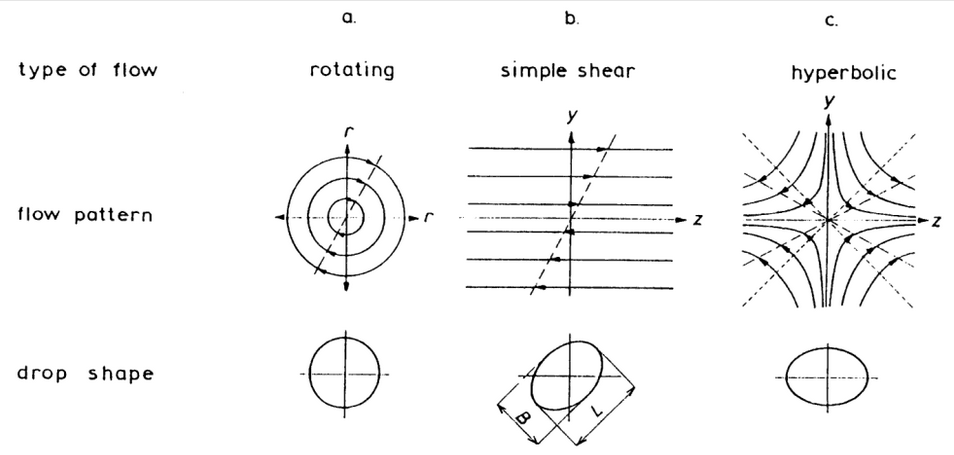
\includegraphics[width=\linewidth]{Markus/Laminarflow}
\end{frame}

\begin{frame}{Laminare Strömung}
	\begin{minipage}{0.7\linewidth}
		\begin{equation*}
		\begin{aligned}
		We_{\,\tx{lam}} &= \frac{\tau}{p_L} = \frac{\tau D}{4 \gamma} \\
		We_{\,\tx{lam, kr}} &= \frac{\tau D_{\tx{max}}}{4 \gamma}
		\end{aligned}
		\end{equation*}
		\vspace{0.5cm}\\
		Viskositätsverhältnis disperse Phase / \\
		Emulsion
		\vspace{0.5cm}
		\begin{equation*}
		0,1 < \frac{\eta_{\tx{d}}}{\eta_{\tx{e}}} < 4
		\end{equation*}
	\end{minipage}%
	\begin{minipage}{0.3\linewidth}
		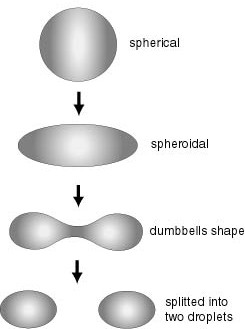
\includegraphics[width=\linewidth]{Markus/liquid_drop_E}
	\end{minipage}
\end{frame}


\begin{frame}{Turbulente Strömung}
	\begin{minipage}{0.4\linewidth}
		\begin{itemize}
			\item Wirbelströme
			\item Trägheitskräfte, turbulente Scherkräfte, viskose Spannungen
		\end{itemize}
	\end{minipage}%
	\begin{minipage}{0.6\linewidth}
		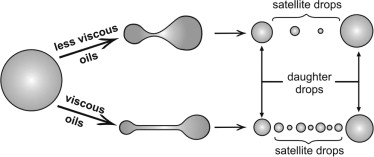
\includegraphics[width=\linewidth]{Markus/turbulentflowdrops}
	\end{minipage}
	\begin{equation*}
	t_{\tx{def}} = \frac{\eta_{\tx{d}}}{\rho_k u'^2 p_K}
	\end{equation*}
	isotrope Turbulenz:
	\begin{equation*}
	D_{\tx{max}} = \rho_c^{-\frac{1}{5}} \gamma^{\frac{3}{5}} P_V^{-\frac{2}{5}}
	\end{equation*}
	$ P_V $ = Leistungsdchte
\end{frame}

\begin{frame}{Kavitation}
	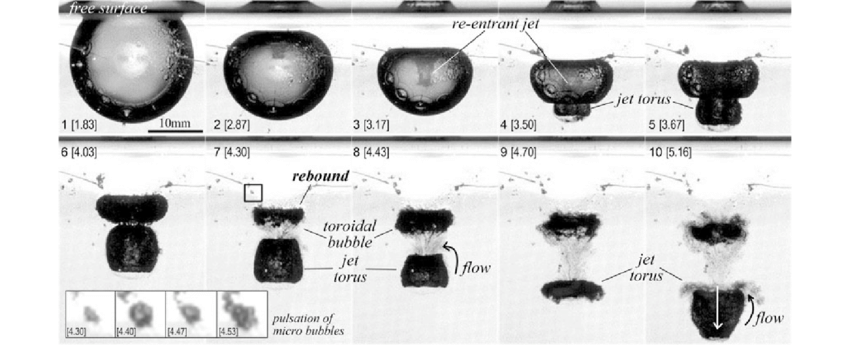
\includegraphics[width=\linewidth]{Markus/Cavitationbubble}
%	\begin{tikzpicture}
%		\draw[color=red!75!black, rounded corners, ultra thick] (-6,0) rectangle (-2,3);
%		\node[shape=rectangle,
%		rounded corners,
%		draw] at (0,0) {testtex der viel zu lange ist};
%	\end{tikzpicture}
\end{frame}

\begin{frame}{Tropfengröße}
	\begin{block}{}
		\begin{itemize}
			\item 0,05 - 100 $ \mu $m
			\item Nano- / Miniemulsionen: 50 - 200 nm
			% Stabilität gegen Auframen oder Sedimentation
			\item Makroemulsion: bis 100 $ \mu $m
			% kleiner als lambda: Durchsichtig oder Opaque. größer: milchig
			\begin{itemize}
				\item Grobdispers: > 1 $ \mu $m
				\item Feindispers: < 1 $ \mu $m
			\end{itemize}
		\end{itemize}
	\end{block}
	\begin{exampleblock}{}
		In Milch: 10 - 30 $ \mu $m\\
		Homogenisierte Milch: 1 - 2 $ \mu $ m
	\end{exampleblock}
\end{frame}

\subsection{Emulgieraparate}

\begin{frame}{Emulgieraparate}
	\begin{block}{}
		\begin{itemize}
			\item Rotor-Stator-Systeme \pause 
			\item Strömungsmechanische Mittel \pause
			\item Ultraschallgeneratoren \pause
			\item Mikrokonstruierte Systeme
		\end{itemize}
	\end{block}
\end{frame}

\begin{frame}{Rotor-Stator-Systeme}
	\hspace{-0.57cm}
	\vspace{1cm}
	\begin{minipage}{0.6\linewidth}
		\centering
		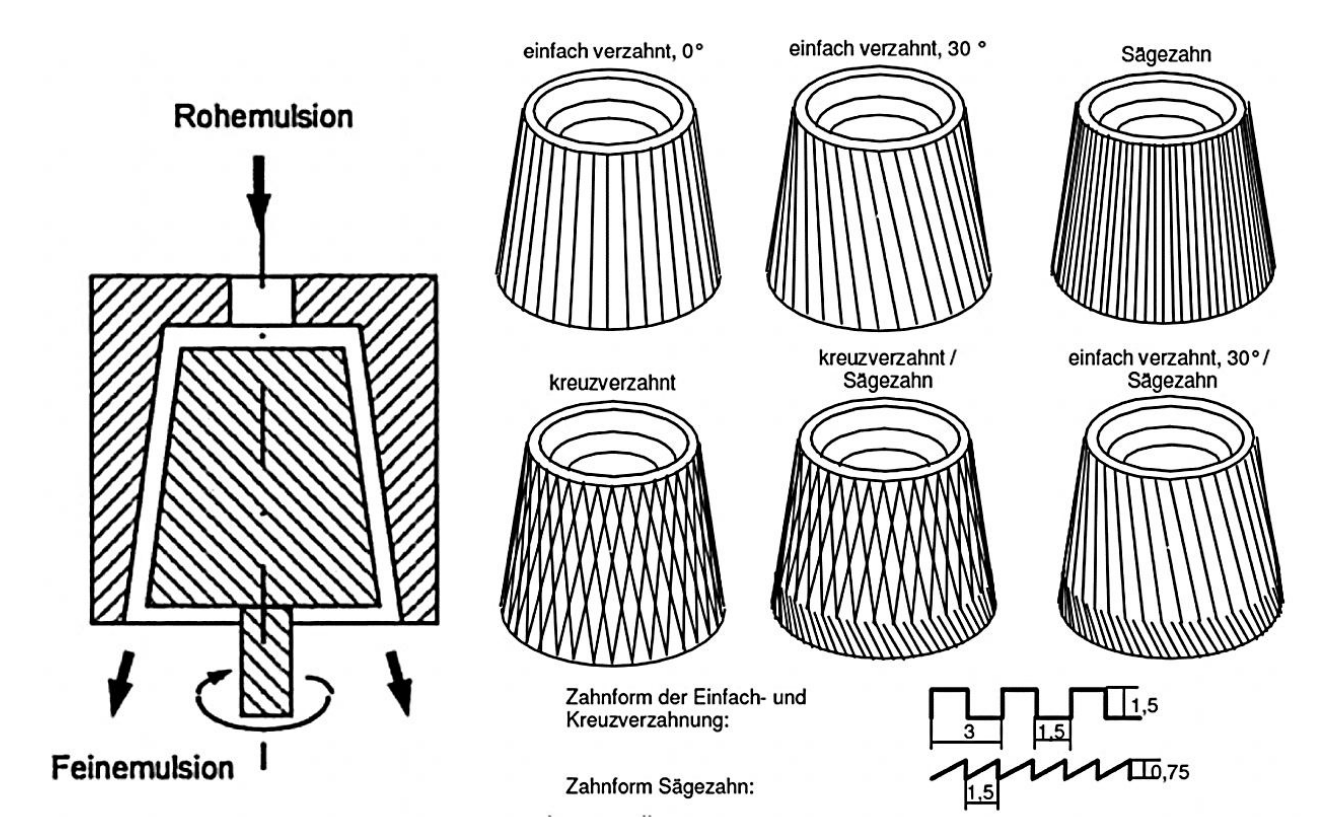
\includegraphics[width=\linewidth]{Markus/Kolloidmuehlen.png}\\
		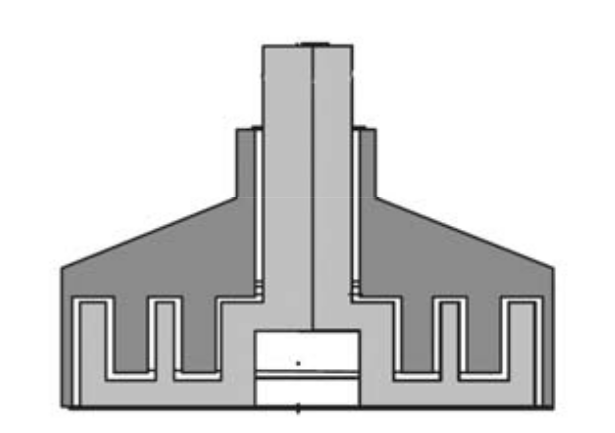
\includegraphics[width=0.7\linewidth]{Markus/Zahnkranzdispergiermaschiene.png}
	\end{minipage}%
	\hspace{-0.3cm}
	\begin{minipage}{0.45\linewidth}
		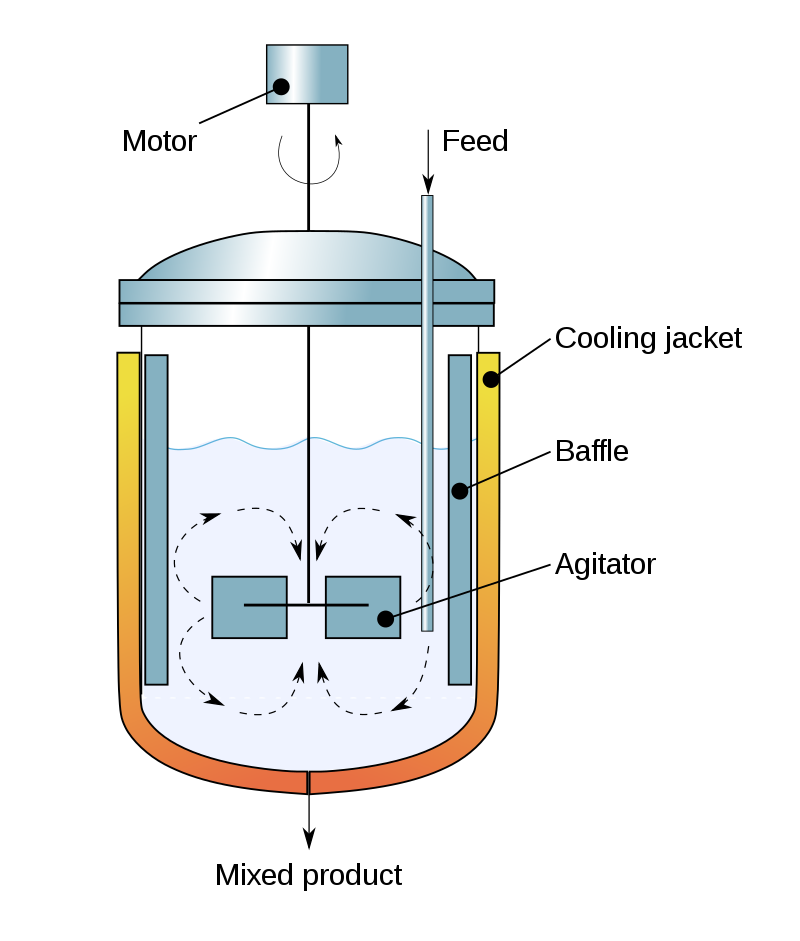
\includegraphics[width=1.1\linewidth]{Markus/Ruehrwerk.png}
	\end{minipage}
\end{frame}

%\begin{frame}{Rotor-Stator-Systeme}
%	\includegraphics*[width=0.5\linewidth]{Markus/Schuettler}
%	\includegraphics*[width=0.5\linewidth]{Markus/Emulgierzentrifuge}
%\end{frame}

\begin{frame}{Strömungsmechanische Mittel}
	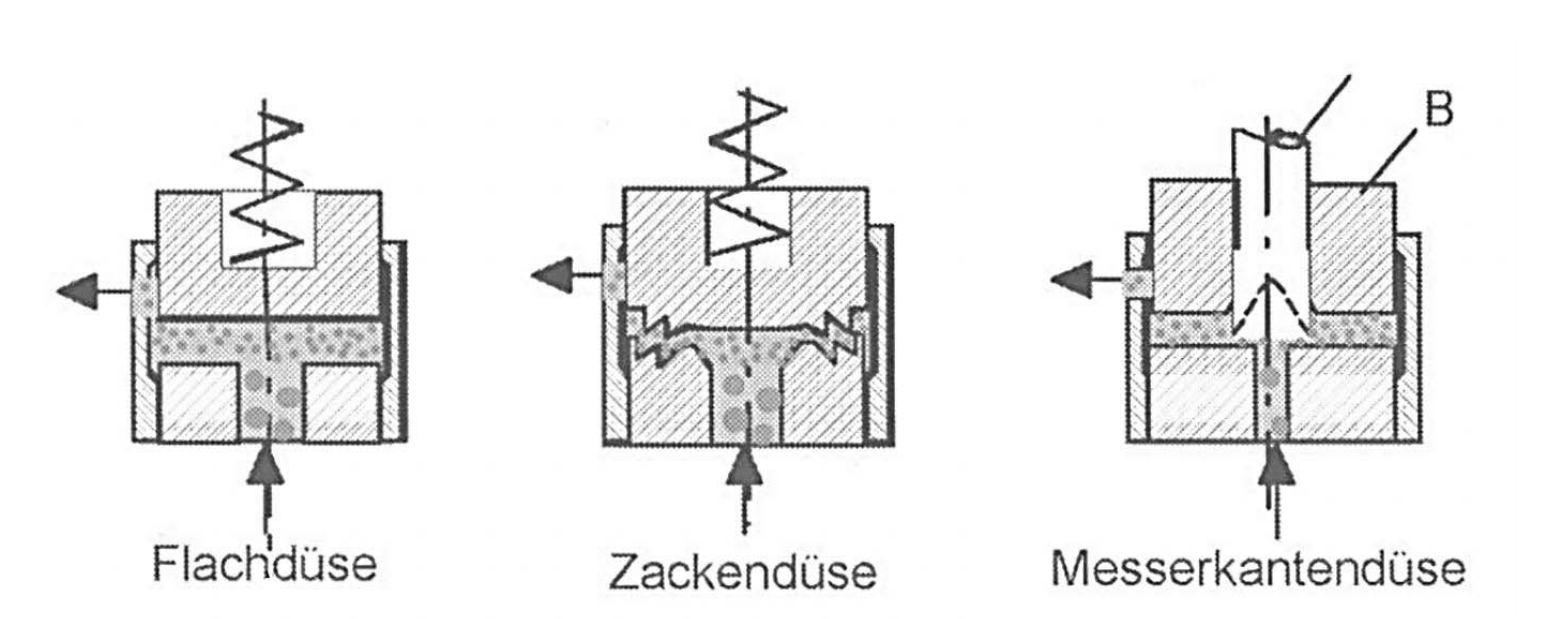
\includegraphics[width=\linewidth]{Markus/Radialdiffusoren}
\end{frame}

\begin{frame}{Ultraschall Homogenisator}
	\centering
	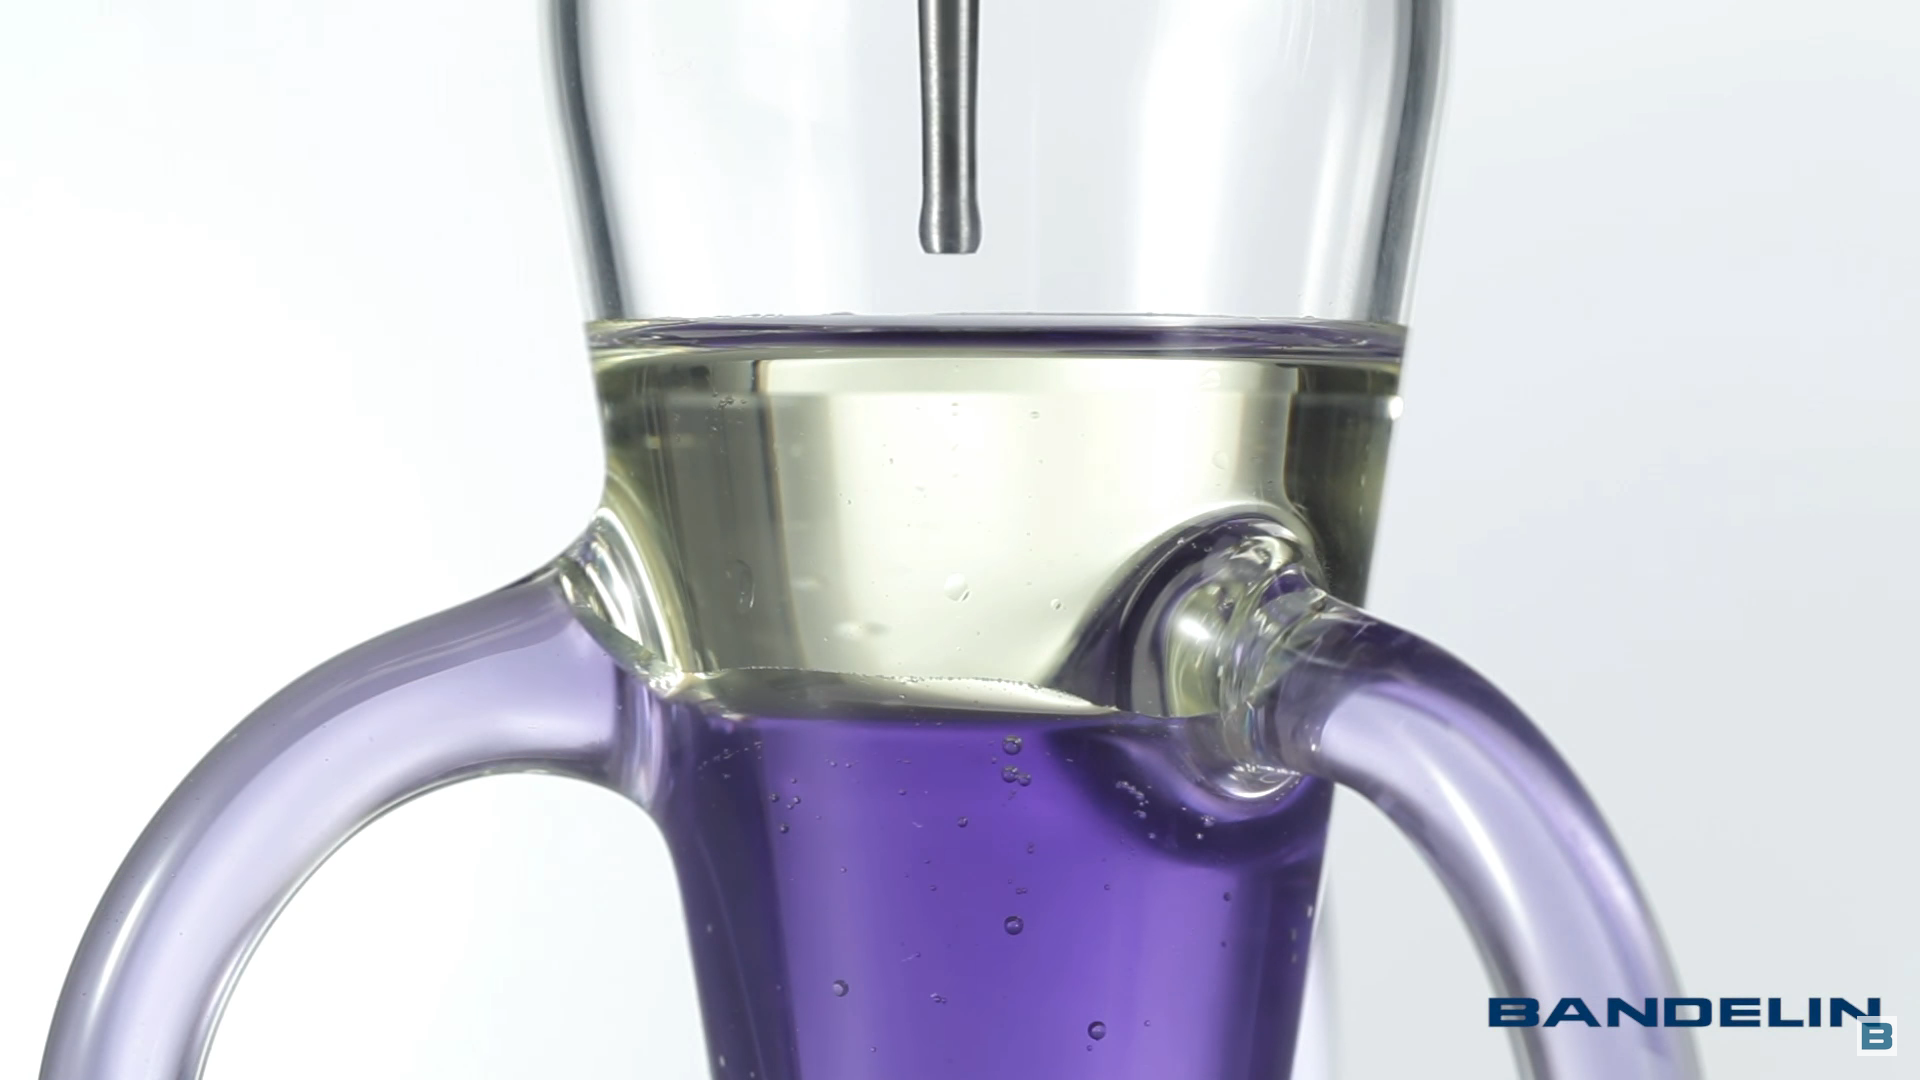
\includegraphics[width=\linewidth]{Markus/uh1}
\end{frame}
\begin{frame}{Ultraschall Homogenisator}
	\centering
	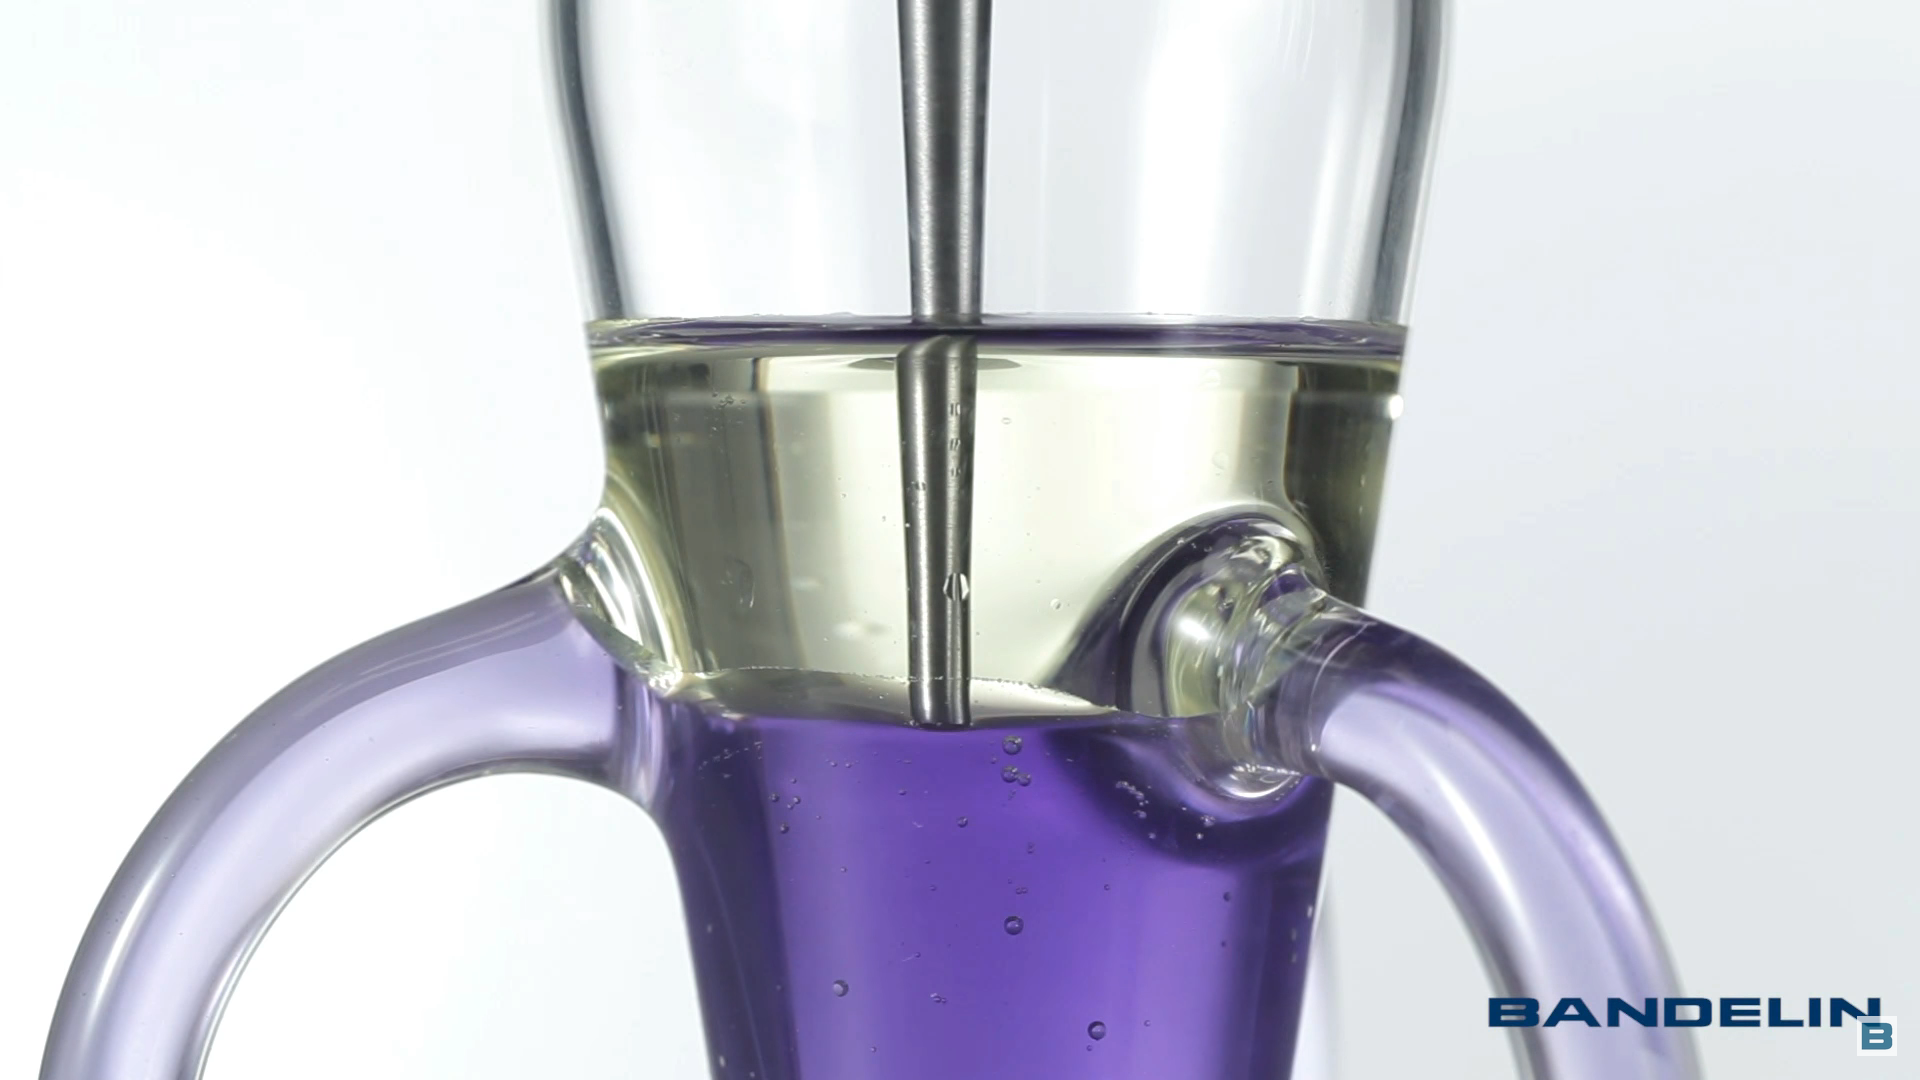
\includegraphics[width=\linewidth]{Markus/uh2}
\end{frame}
\begin{frame}{Ultraschall Homogenisator}
	\centering
	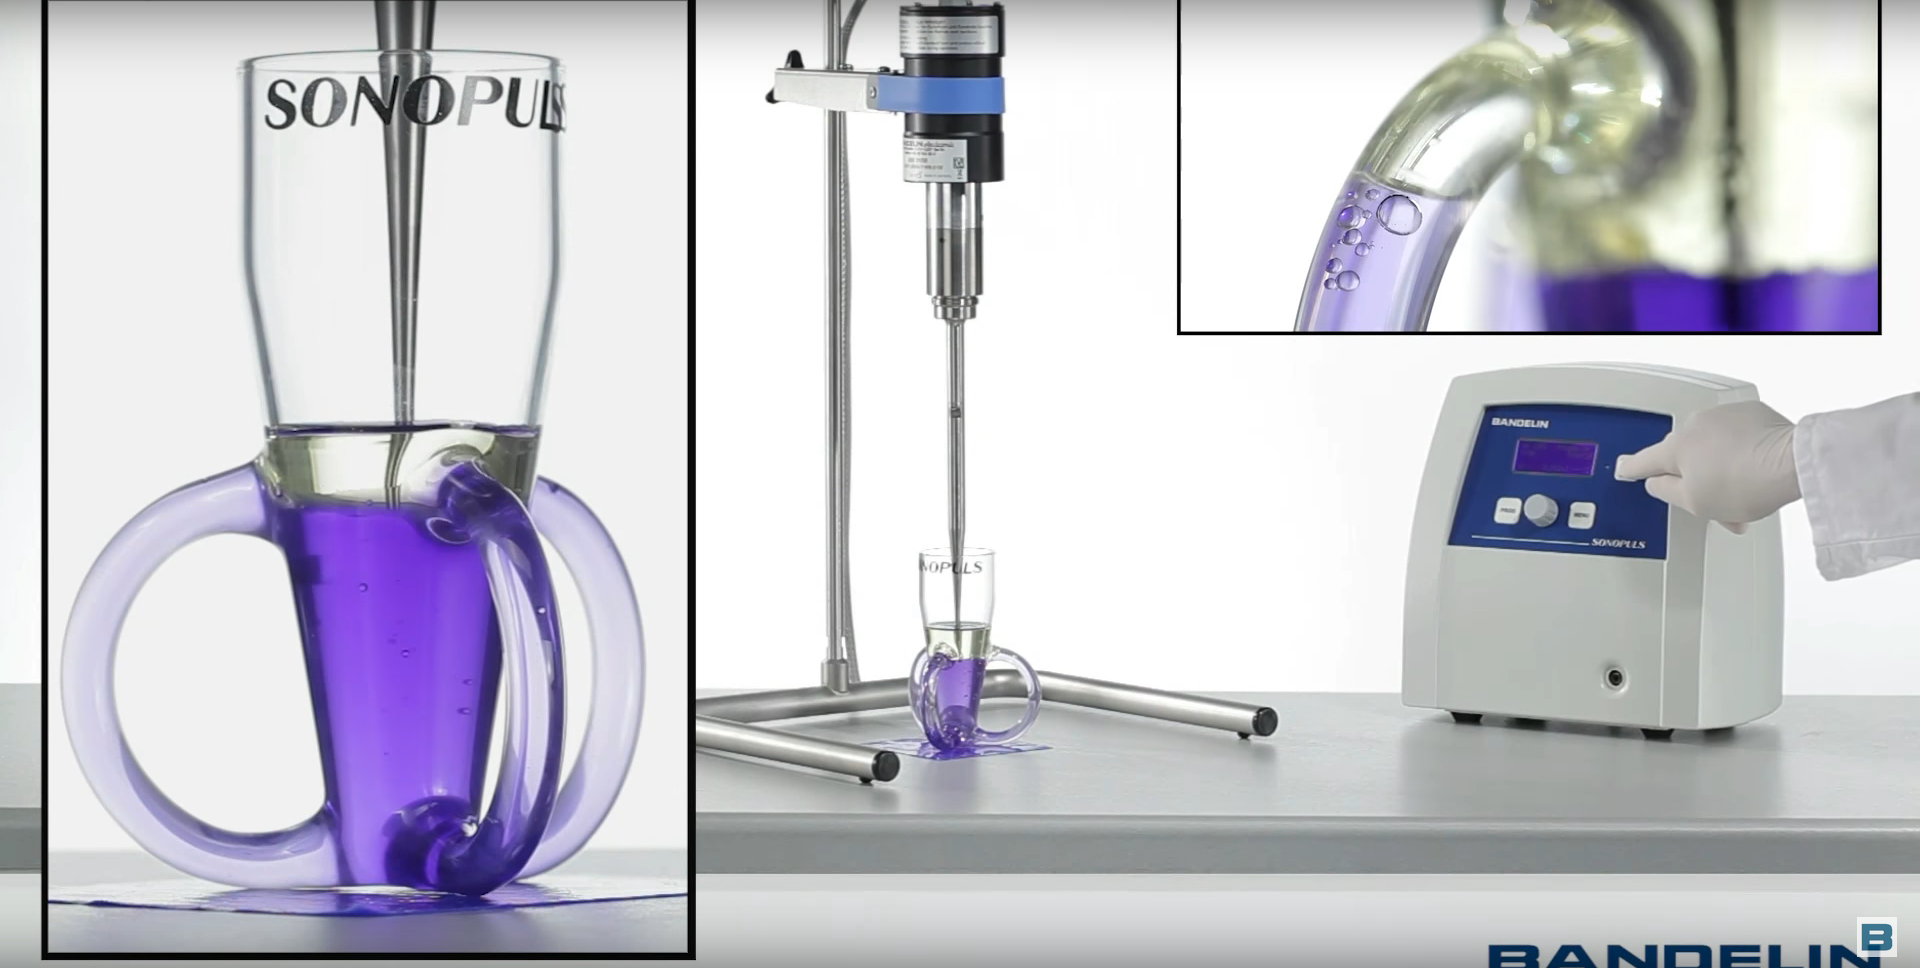
\includegraphics[width=\linewidth]{Markus/uh3}
\end{frame}
\begin{frame}{Ultraschall Homogenisator}
	\centering
	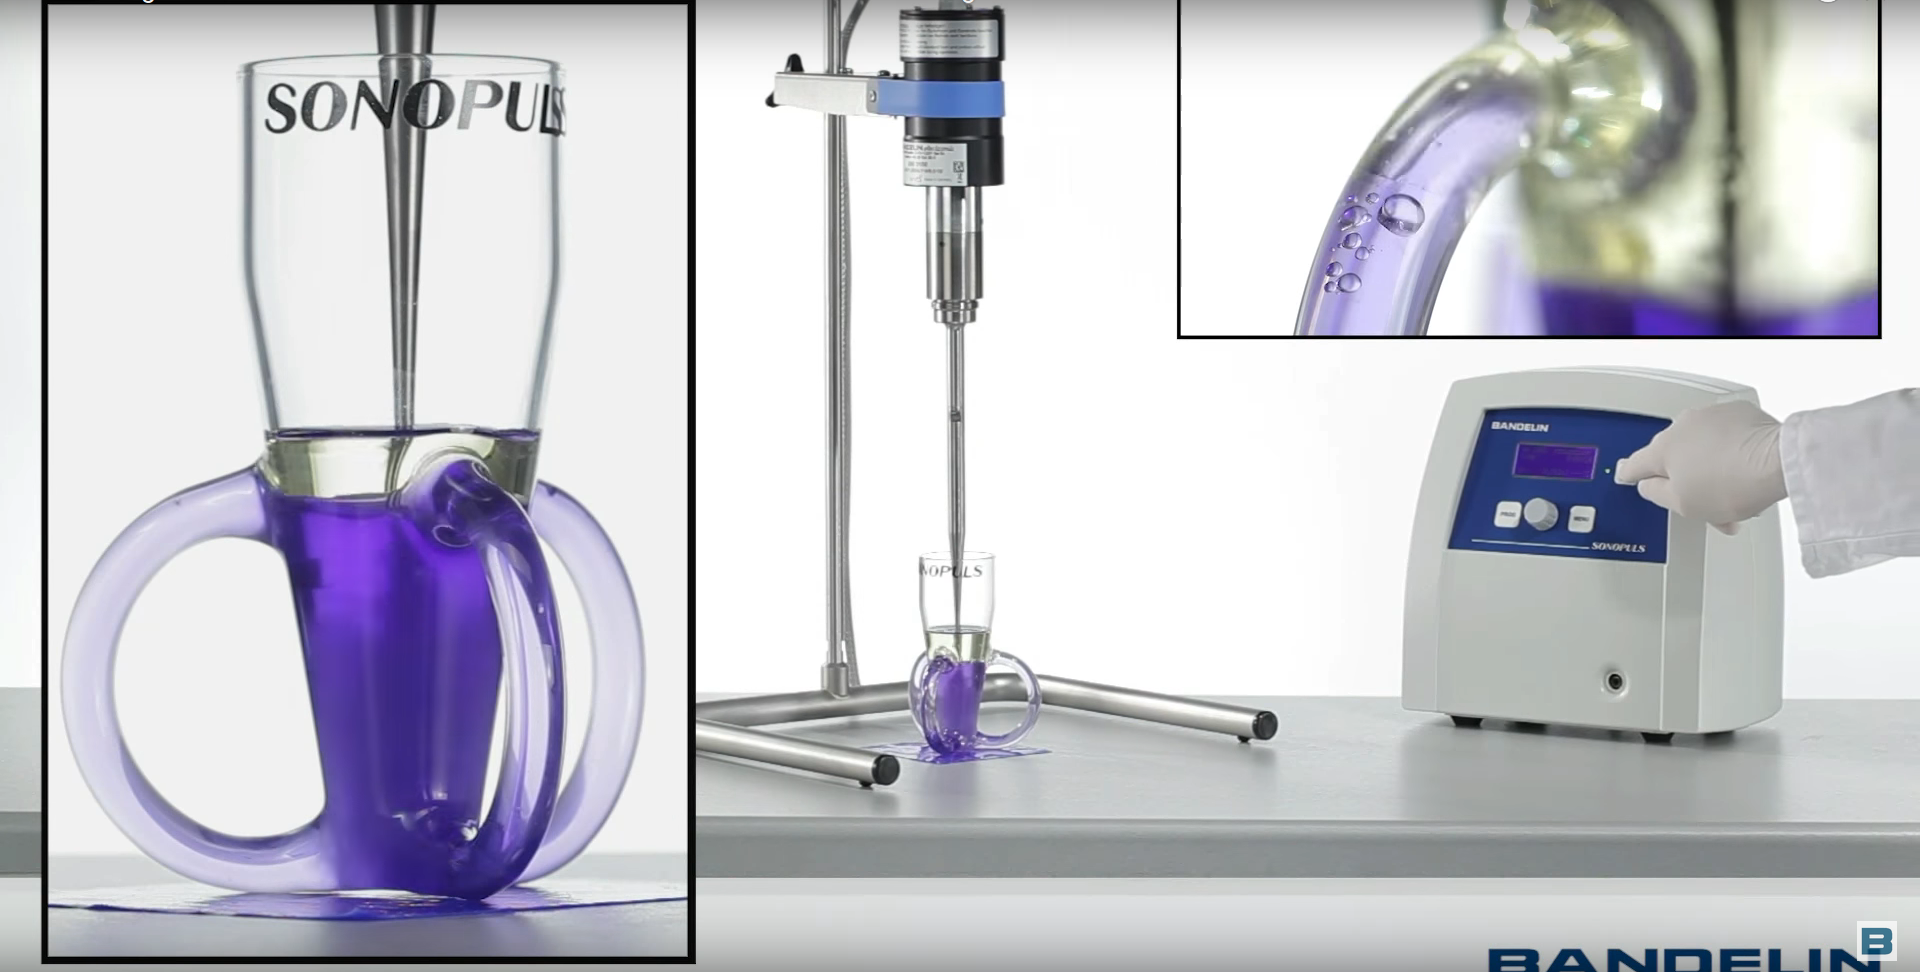
\includegraphics[width=\linewidth]{Markus/uh4}
\end{frame}
\begin{frame}{Ultraschall Homogenisator}
	\centering
	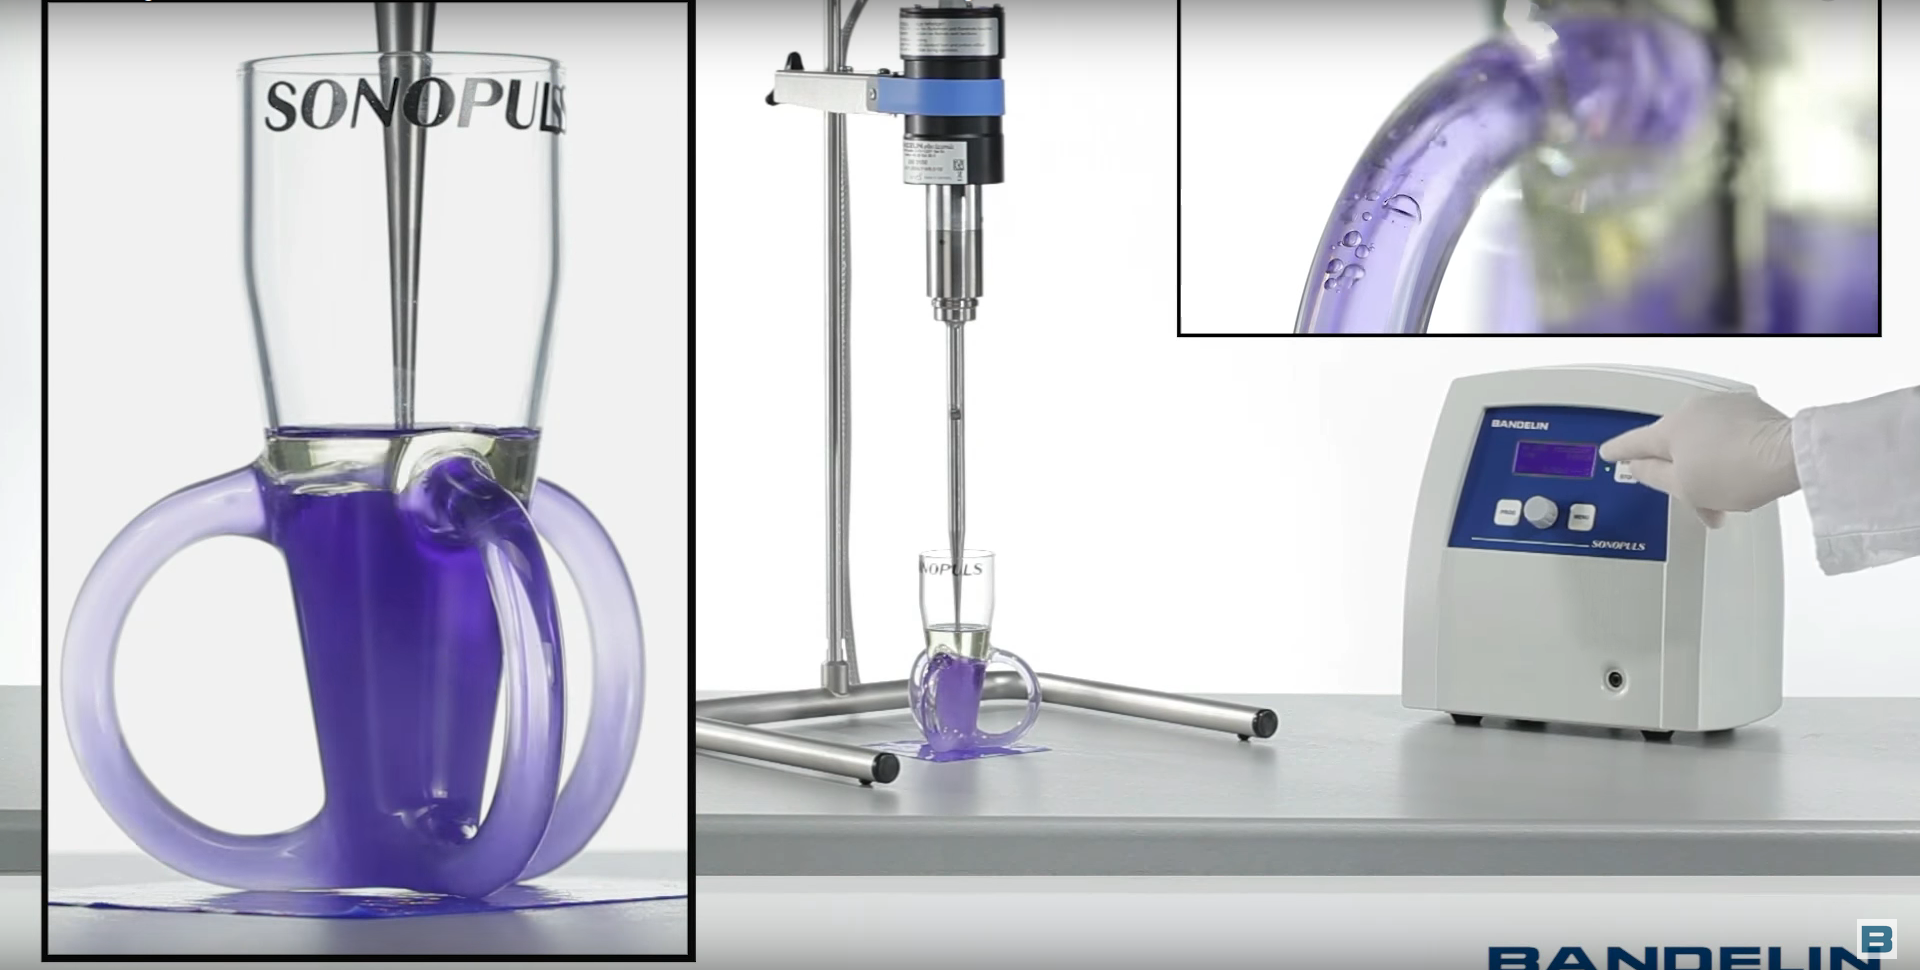
\includegraphics[width=\linewidth]{Markus/uh5}
\end{frame}
\begin{frame}{Ultraschall Homogenisator}
	\centering
	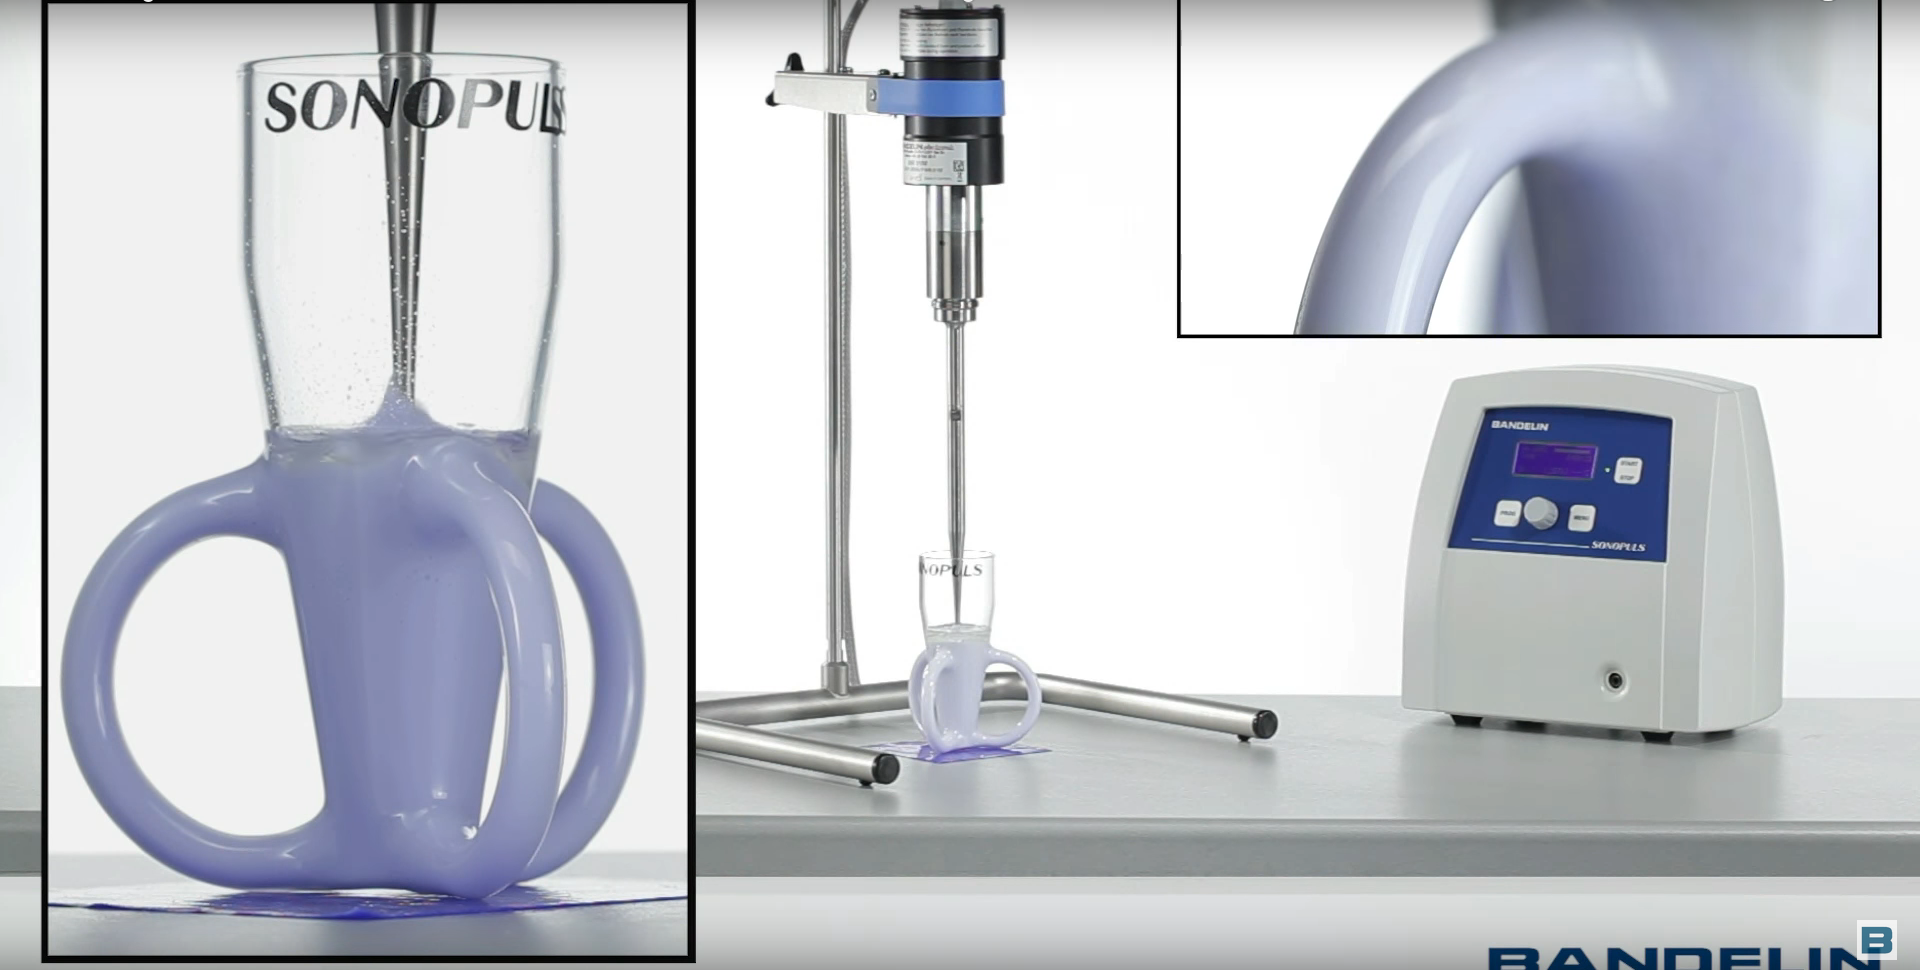
\includegraphics[width=\linewidth]{Markus/uh6}
\end{frame}

\begin{frame}{Anwendung: Salatdressing - Vinaigrette}
	\flushright
	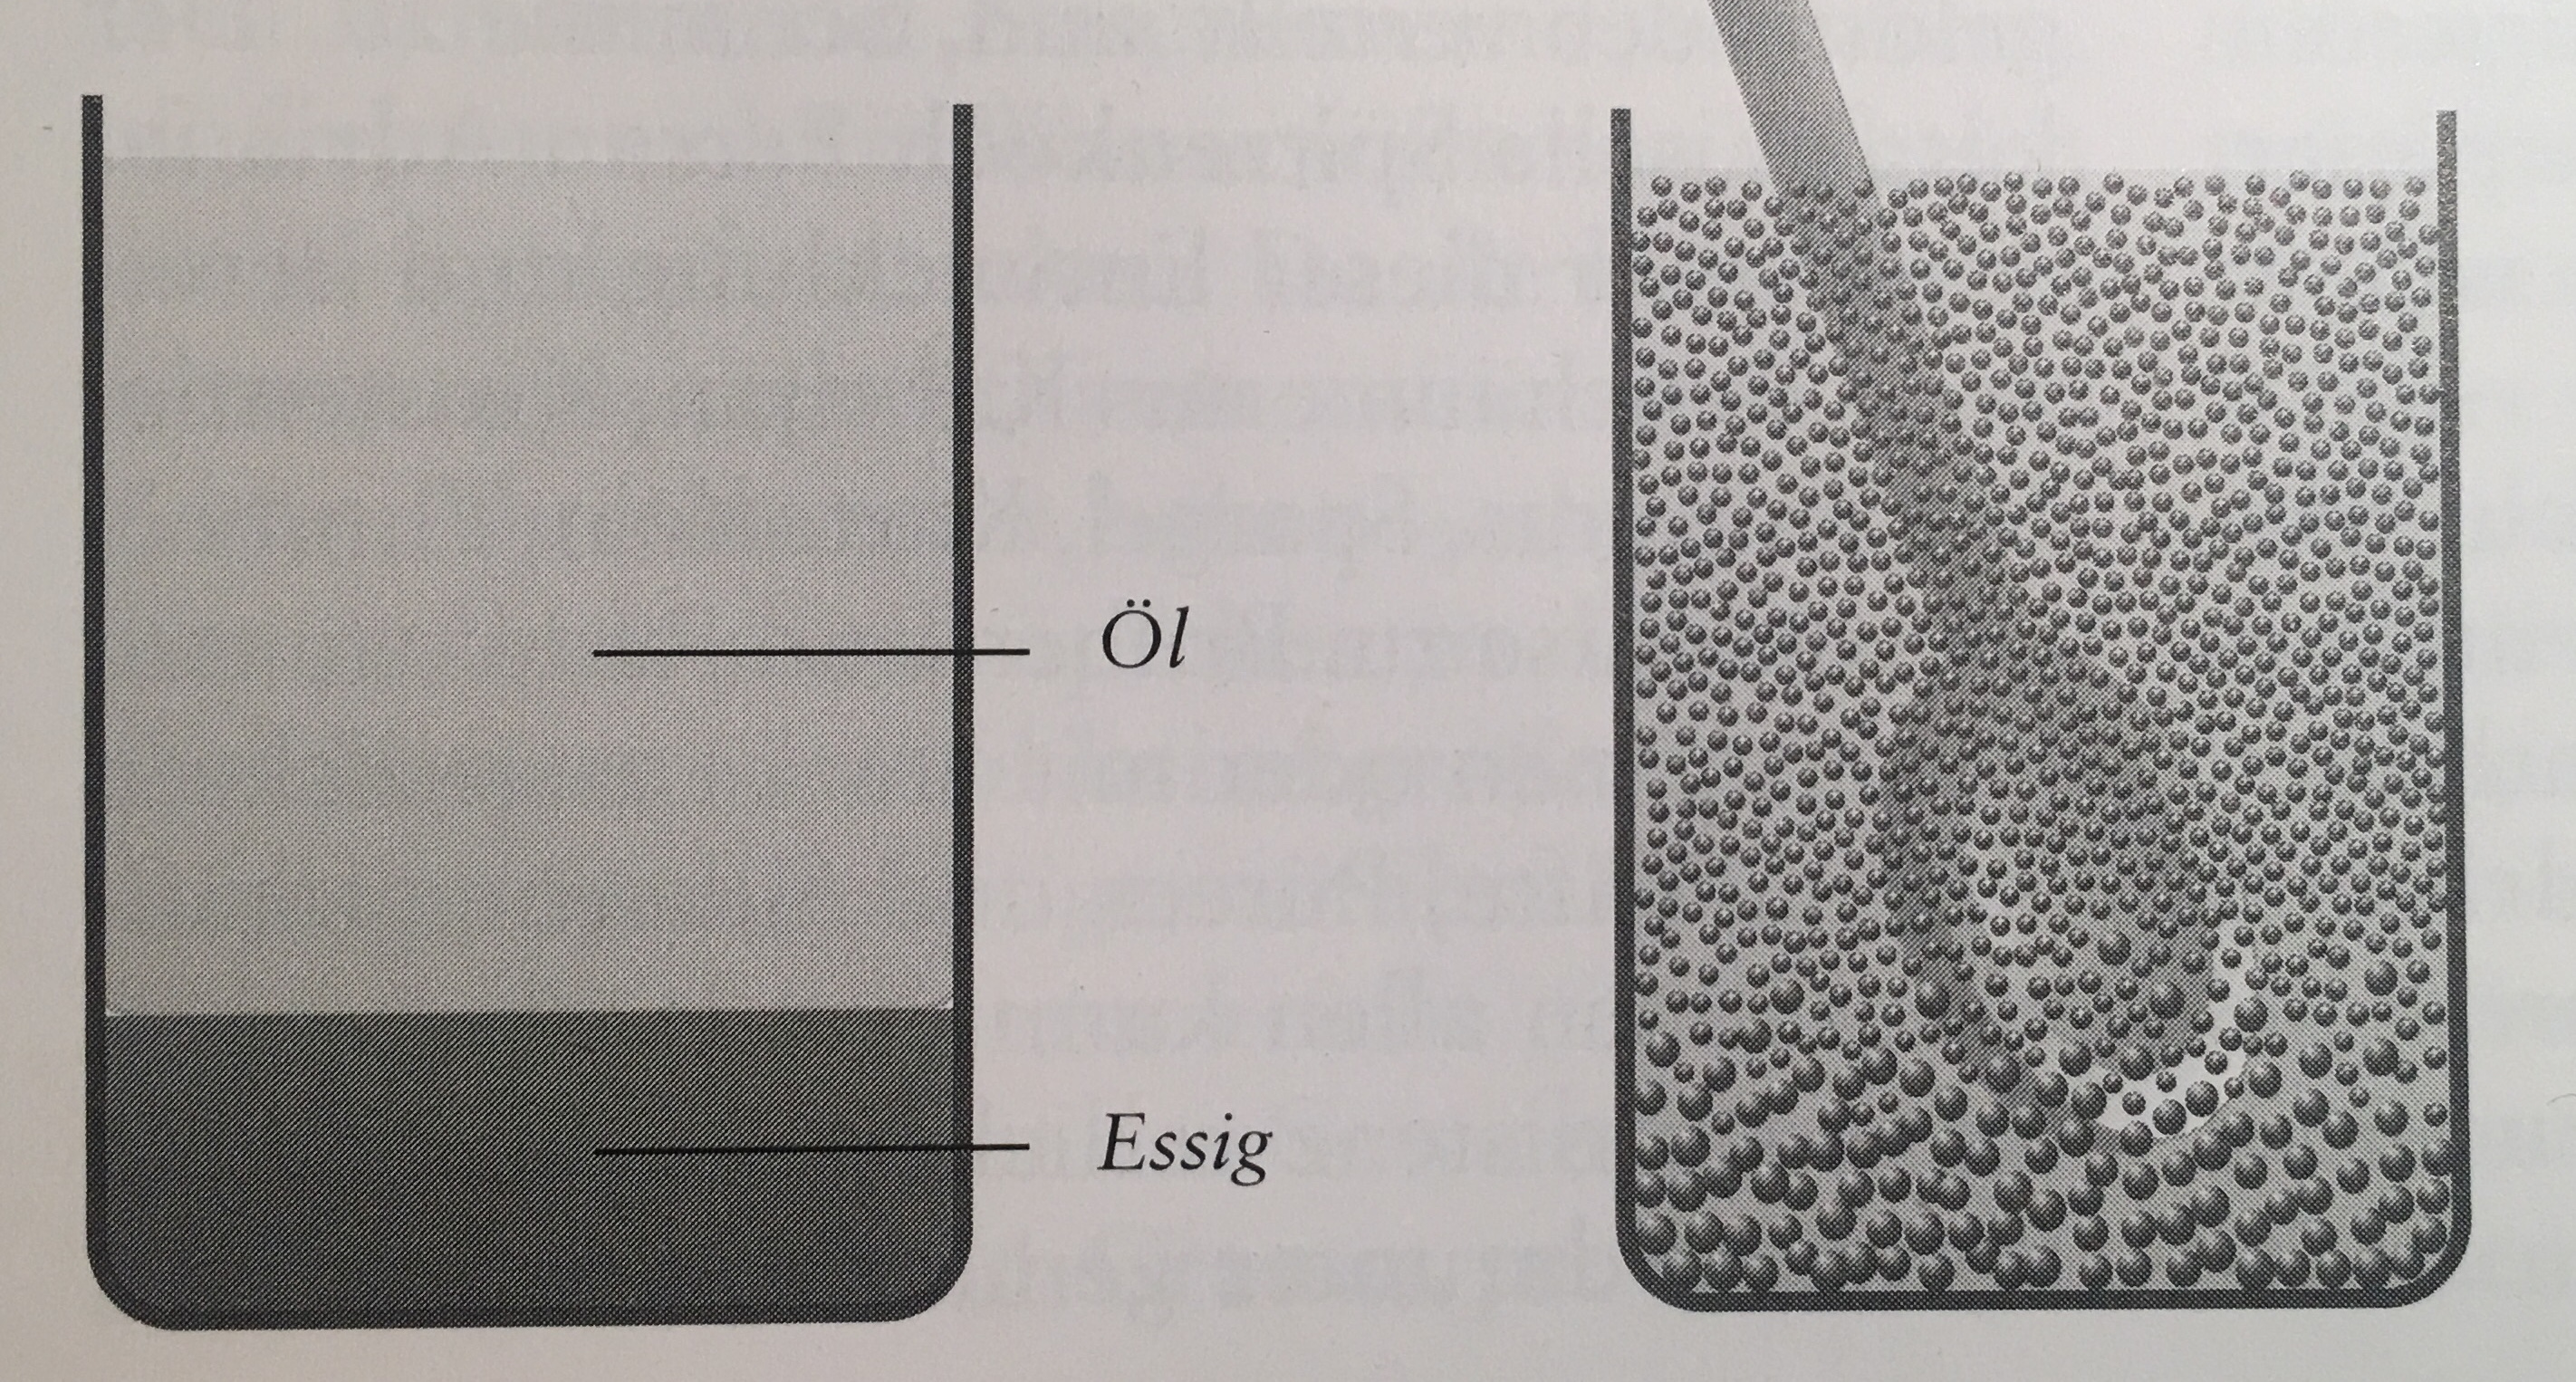
\includegraphics[width=0.6\linewidth]{Markus/Vinaigrette}
	\flushleft
	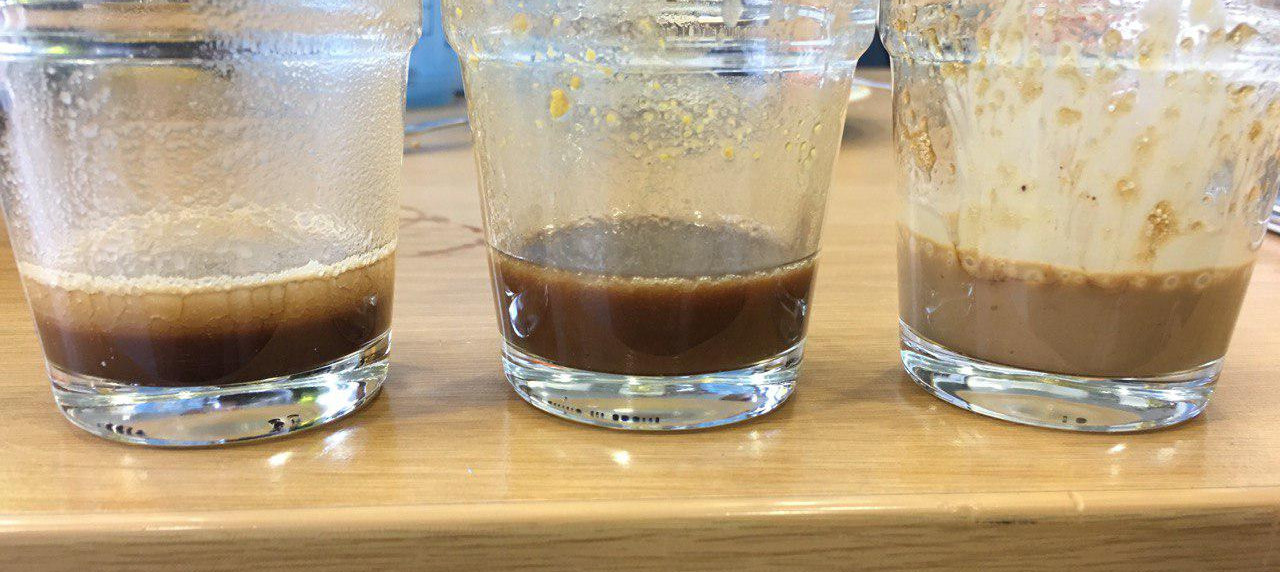
\includegraphics[width=0.6\linewidth]{Markus/Vinaigrette_test}
\end{frame}


%Phillip?:

\section{Emulgatoren}
\begin{frame}
\frametitle{Emulgatoren}
\begin{figure}
\centering
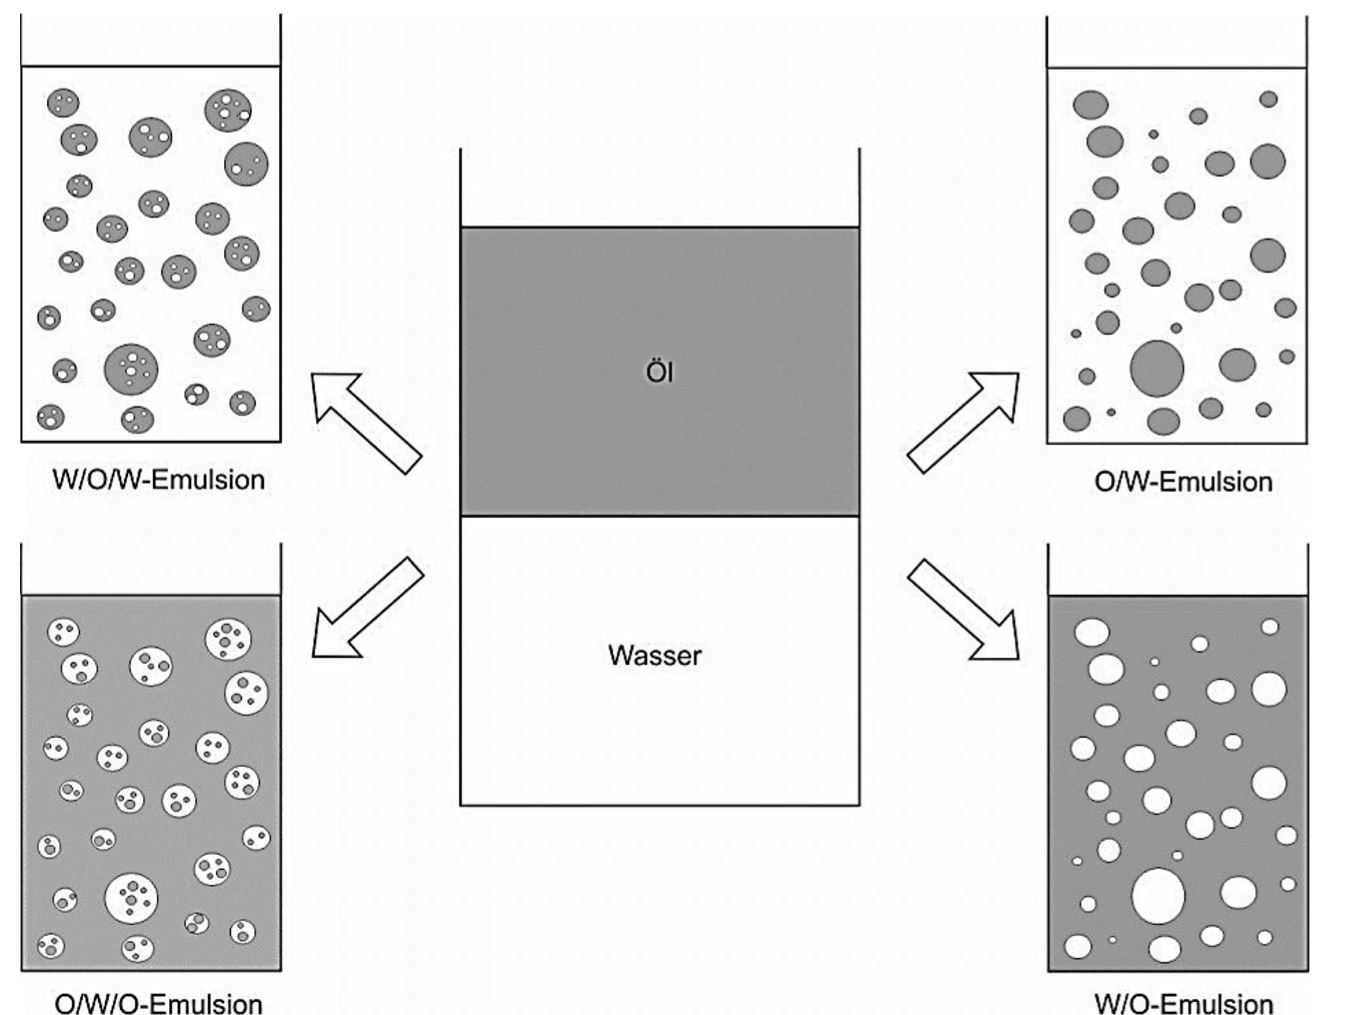
\includegraphics[width = 0.7\textwidth]{Emulsionsarten.JPG}
\caption{Emulsionen von Wasser und Öl}
\end{figure}
\begin{block}{}
Erhöhte Stabilität gegen Aufrahmen bzw. Sedimentation
\end{block}
\end{frame}

\begin{frame}
\frametitle{Emulgatoren}
\begin{figure}
\centering
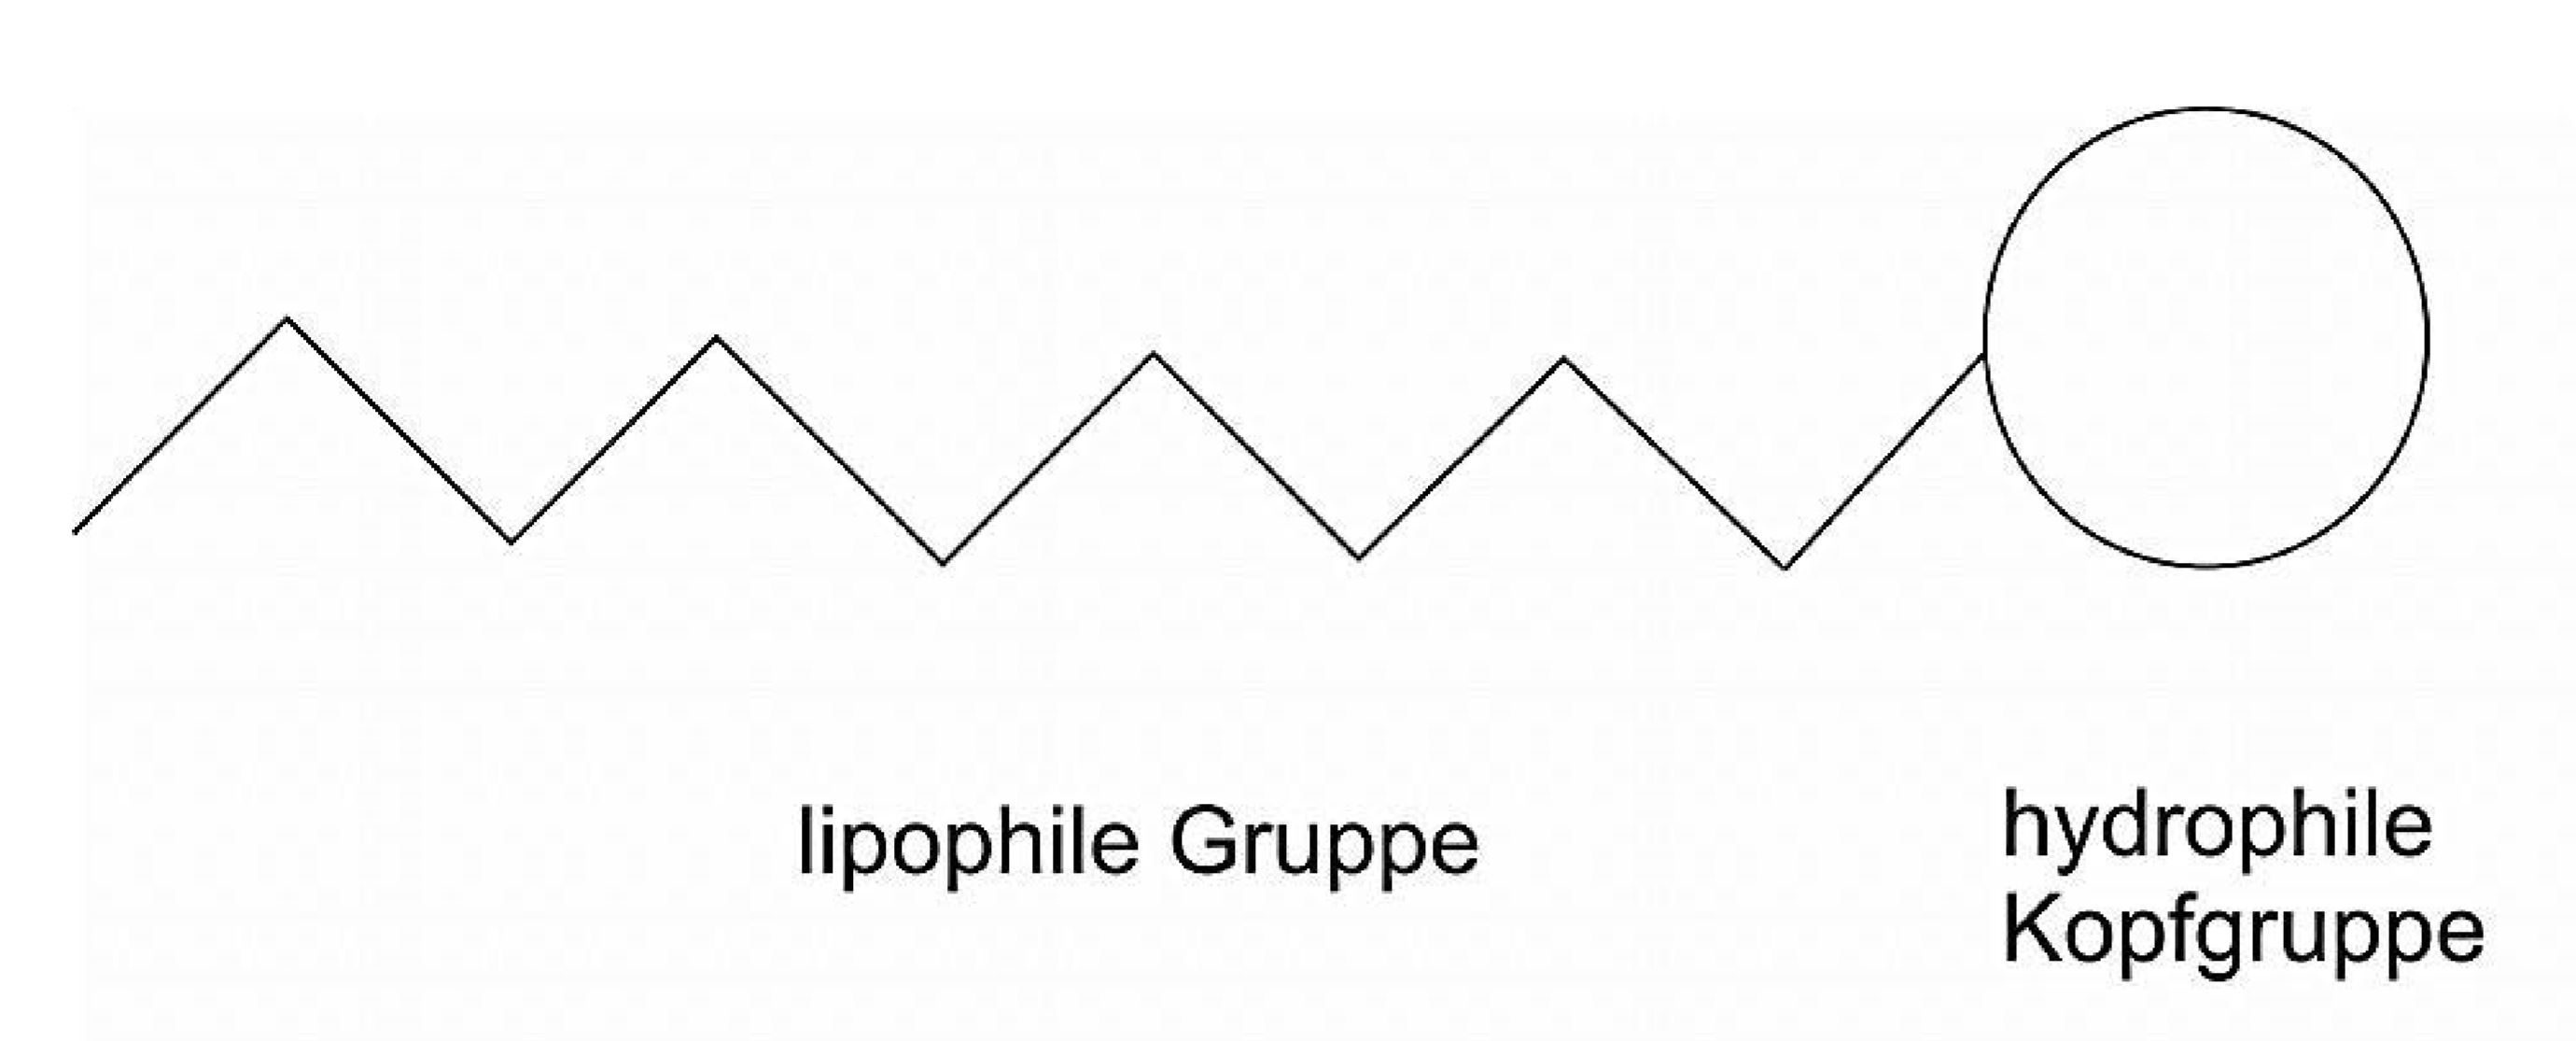
\includegraphics[width = 0.7\textwidth]{EmulgatorAllgemein.JPG}
\end{figure}
\end{frame}

\subsection{Beispiel Lecitin}

\begin{frame}
\frametitle{Beispiel: Lecithin (E322)}
\begin{block}{}
Gemisch unterschiedlicher polarer Lipide (Fette)
\end{block}
\begin{figure}
\centering
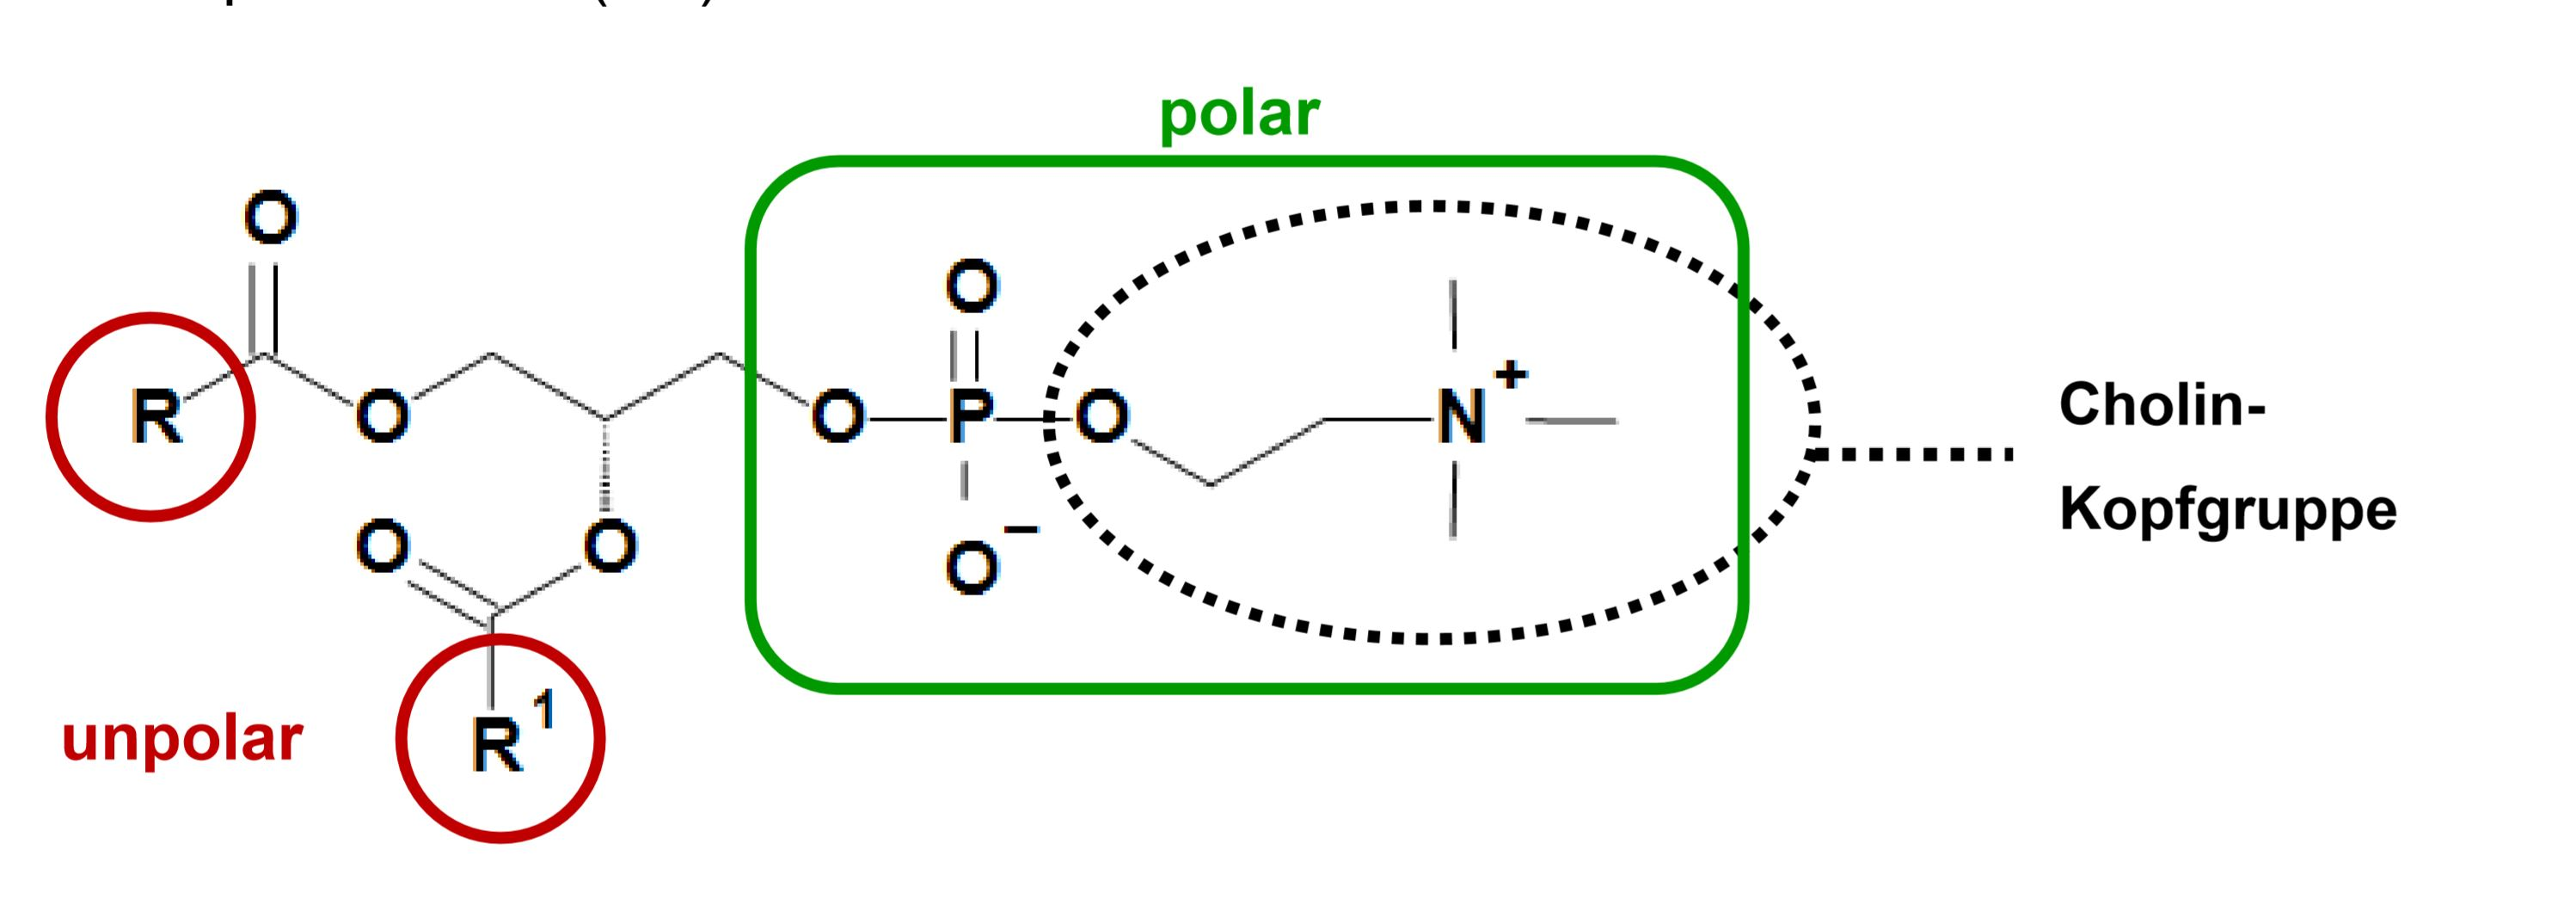
\includegraphics[width = 0.9\textwidth]{Lecithin.JPG}
\caption{Plospholipid (PL), genauer Phosphatidylcholin (PC) }
\end{figure}
\pause
\begin{figure}[H]
\centering
\begin{subfigure}[c]{0.5\textwidth}
\centering
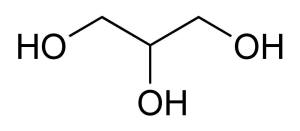
\includegraphics[width = 0.5\textwidth]{glycerol.jpg}
\end{subfigure}
\begin{subfigure}[c]{0.45\textwidth}
\centering
Glycerol, Propan-1,2,3-triol
%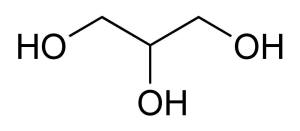
\includegraphics[width = 0.3\textwidth]{glycerol.jpg}
\end{subfigure}
\end{figure}
\end{frame}

\begin{frame}
\frametitle{Beispiel: Lecithin (E322)}
\begin{figure}
\centering
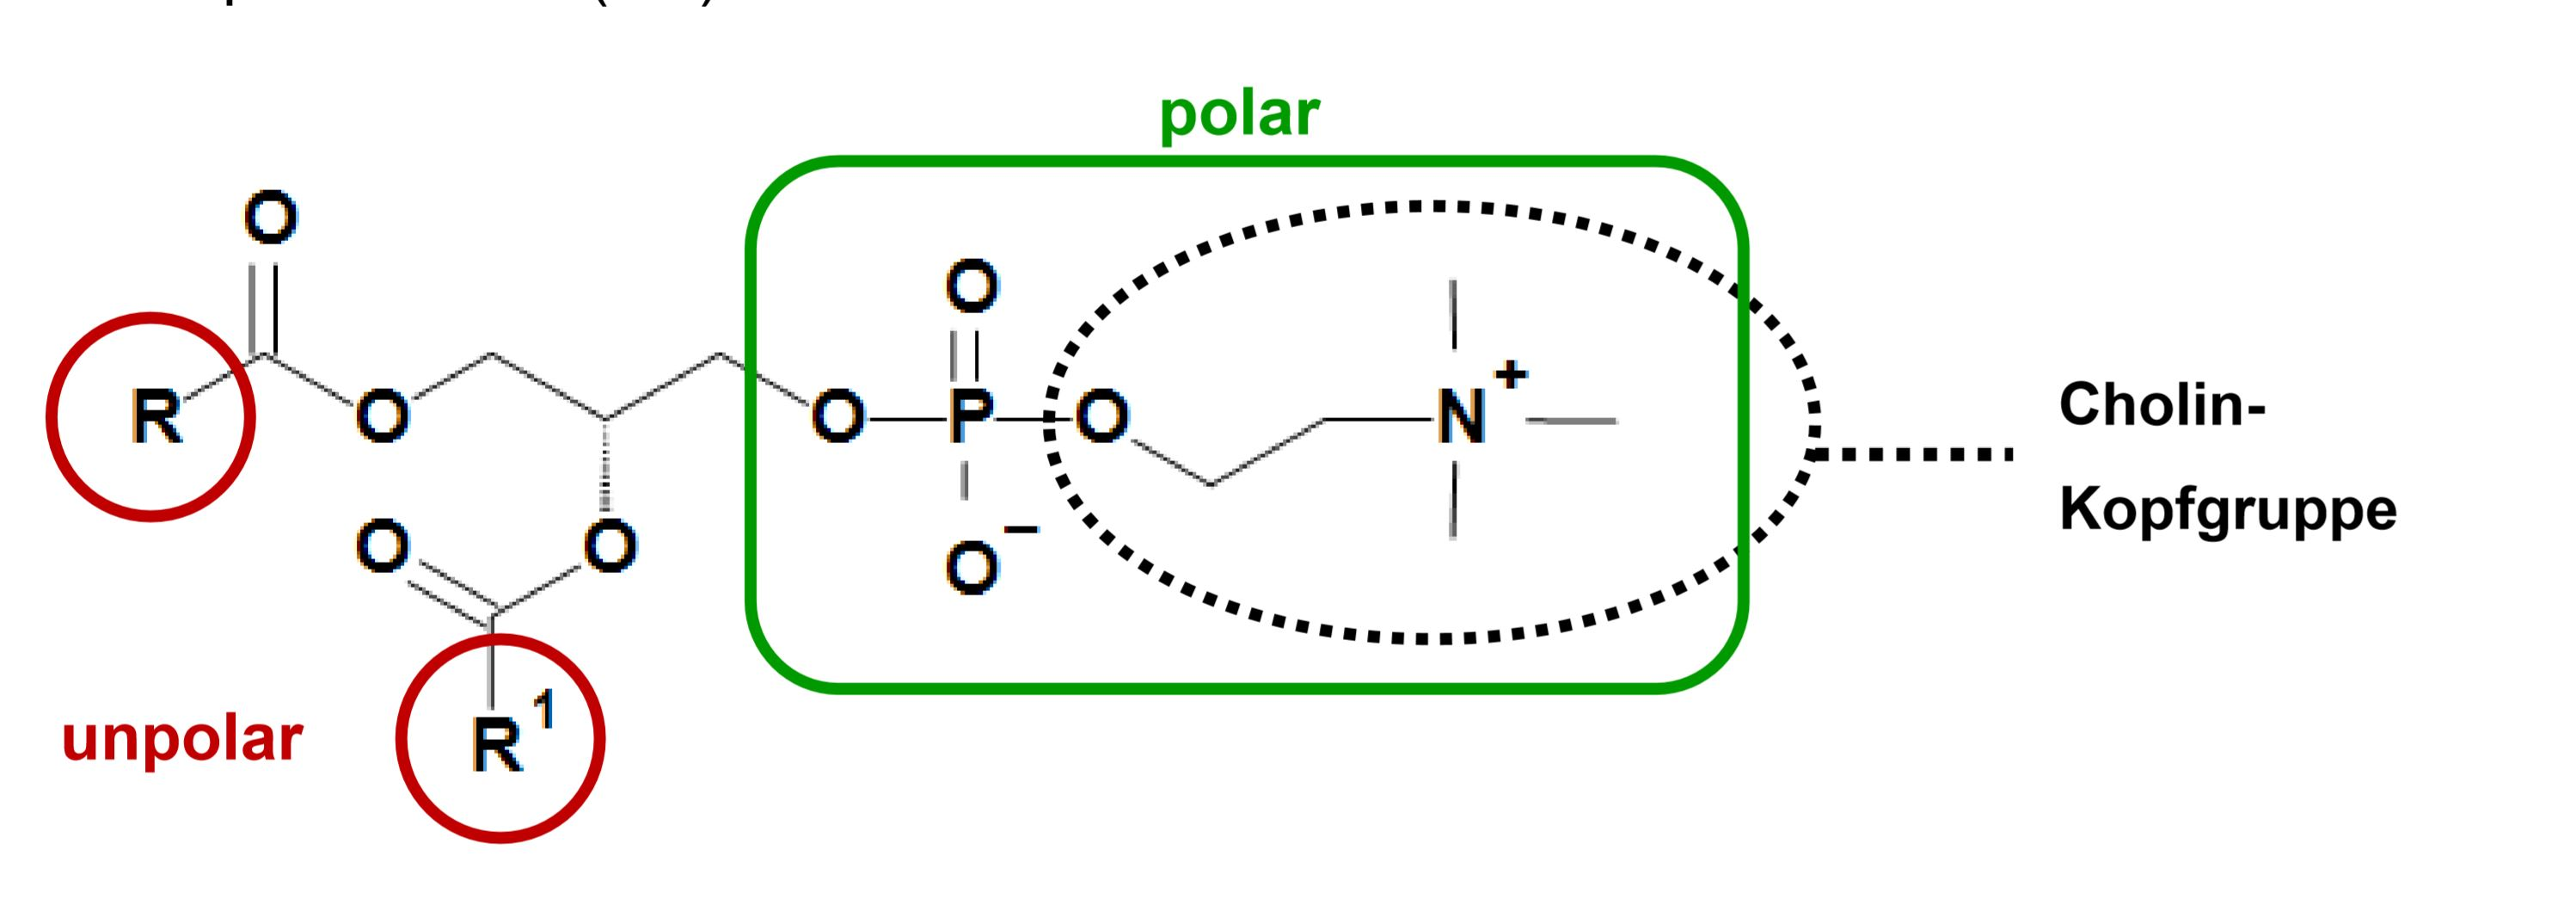
\includegraphics[width = 0.9\textwidth]{Lecithin.JPG}
\caption{Plospholipid (PL), genauer Phosphatidylcholin (PC) }
\end{figure}
Weitere Kopfgruppen:
\begin{figure}[h]
\centering
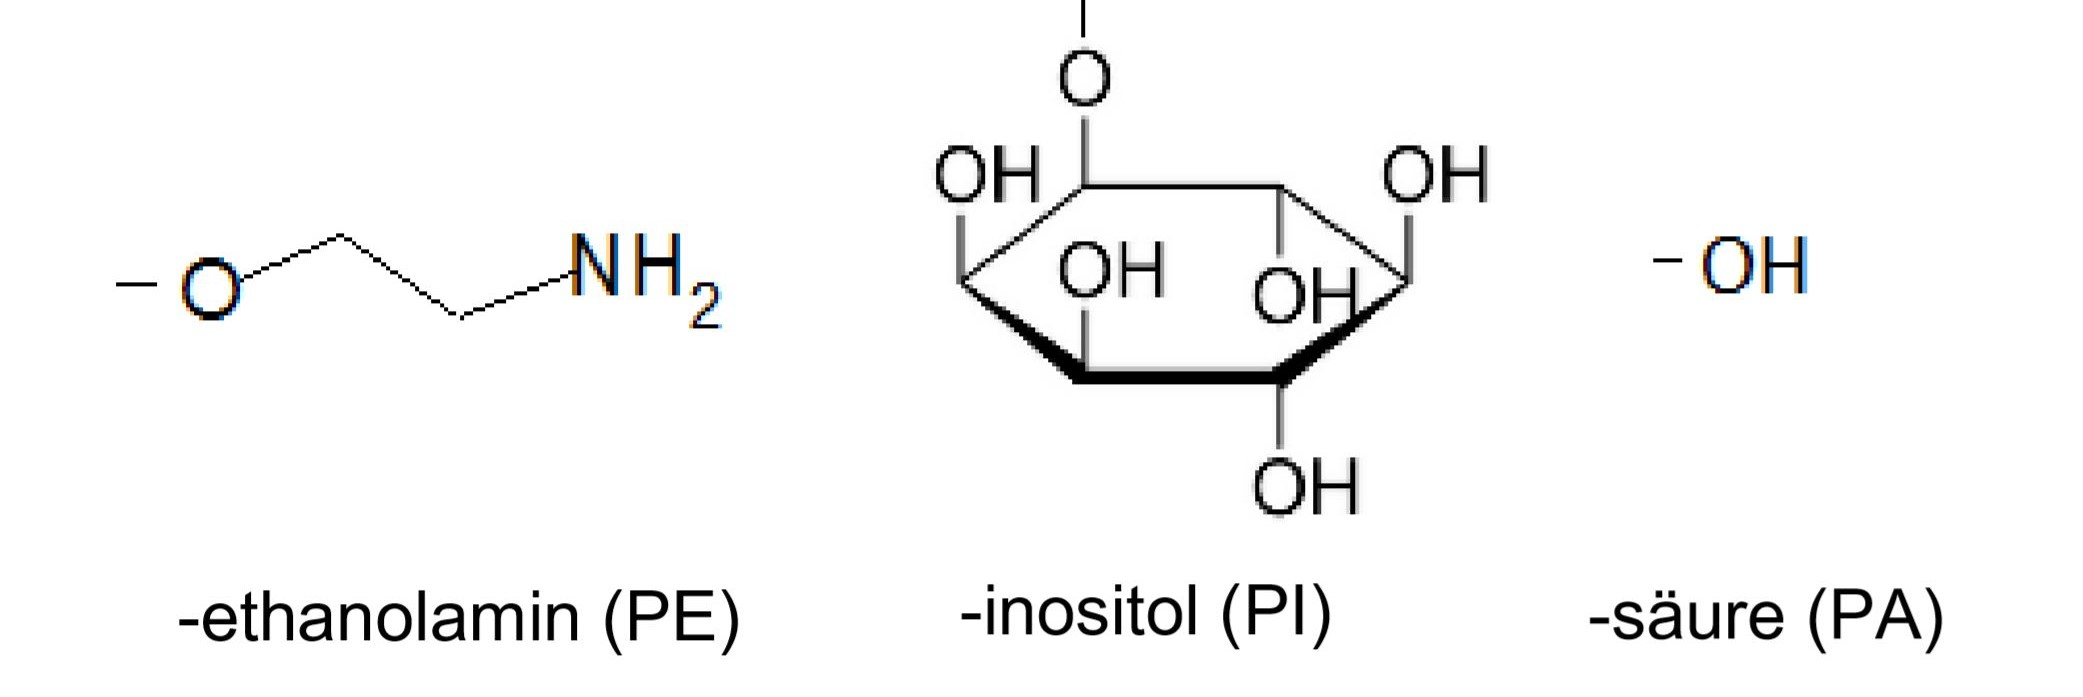
\includegraphics[width = 0.8\textwidth]{Kopfgruppen.JPG}
\end{figure}
\end{frame}

\begin{frame}
\frametitle{Beispiel: Lecithin (E322)}
\begin{figure}
\centering
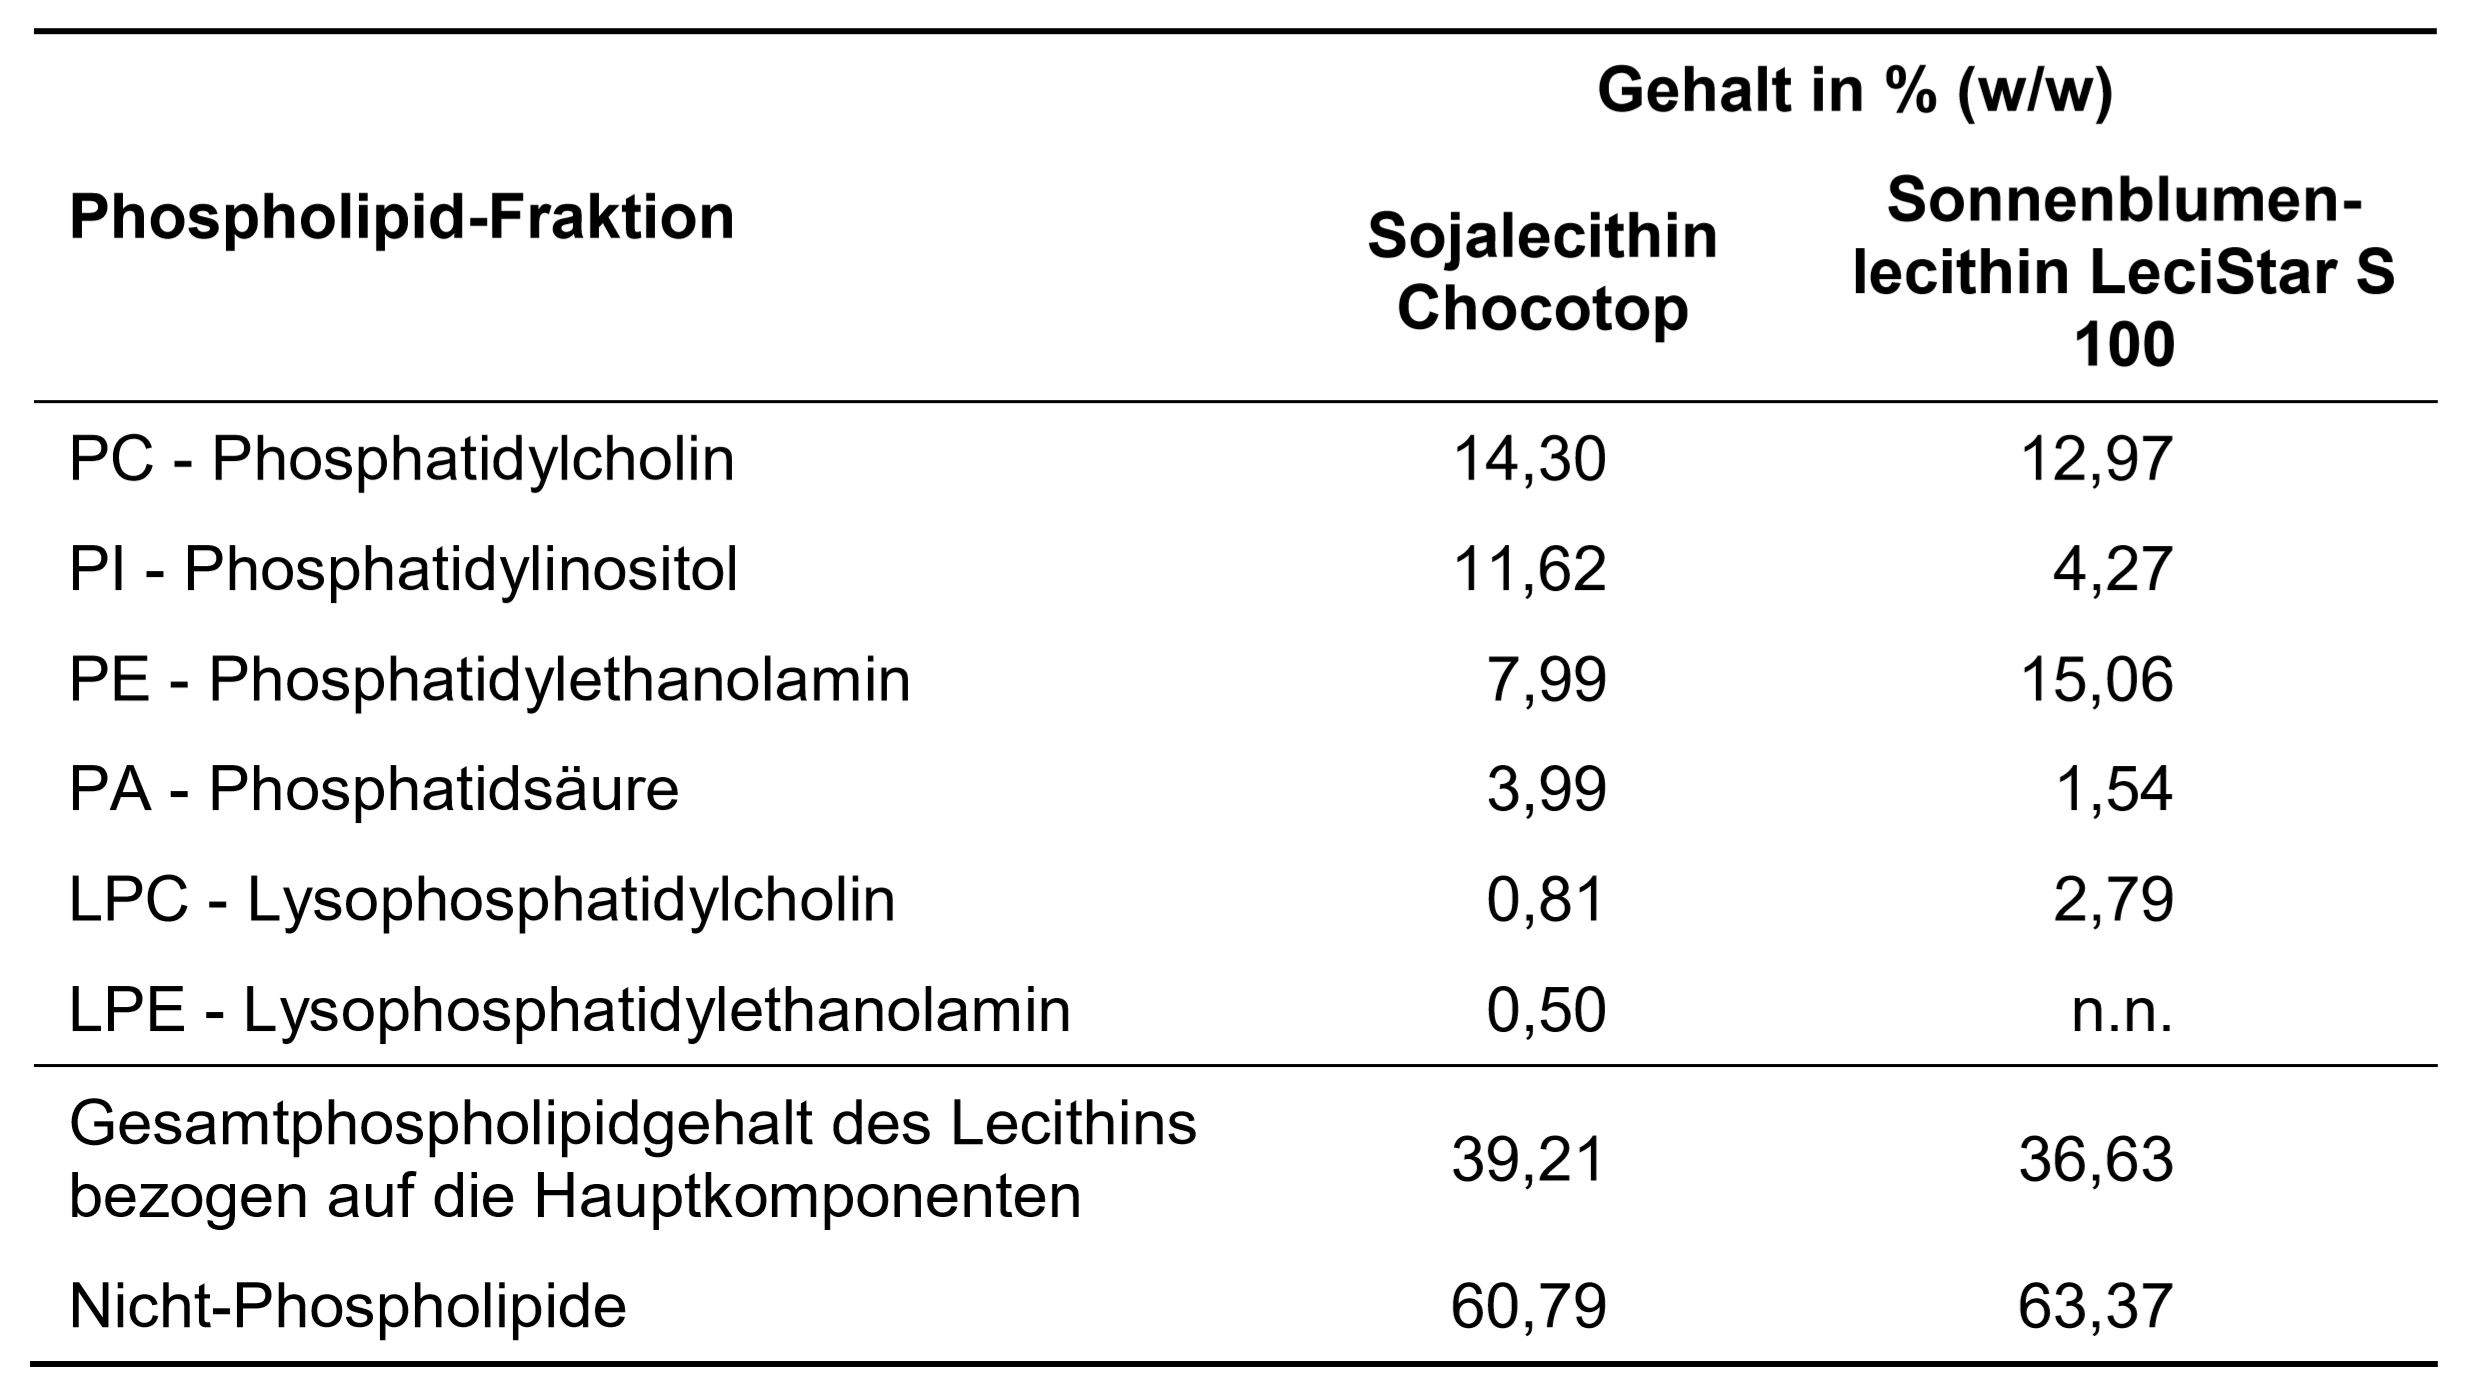
\includegraphics[width = 0.9\textwidth]{ZusammensetzungLecithin.JPG}
\caption{Zusammensetzung Lecithin}
\end{figure}
\end{frame}

%\begin{frame}
%Optionale Folie
%\begin{figure}
%\frametitle{Nicht Phospholipide}
%\centering
%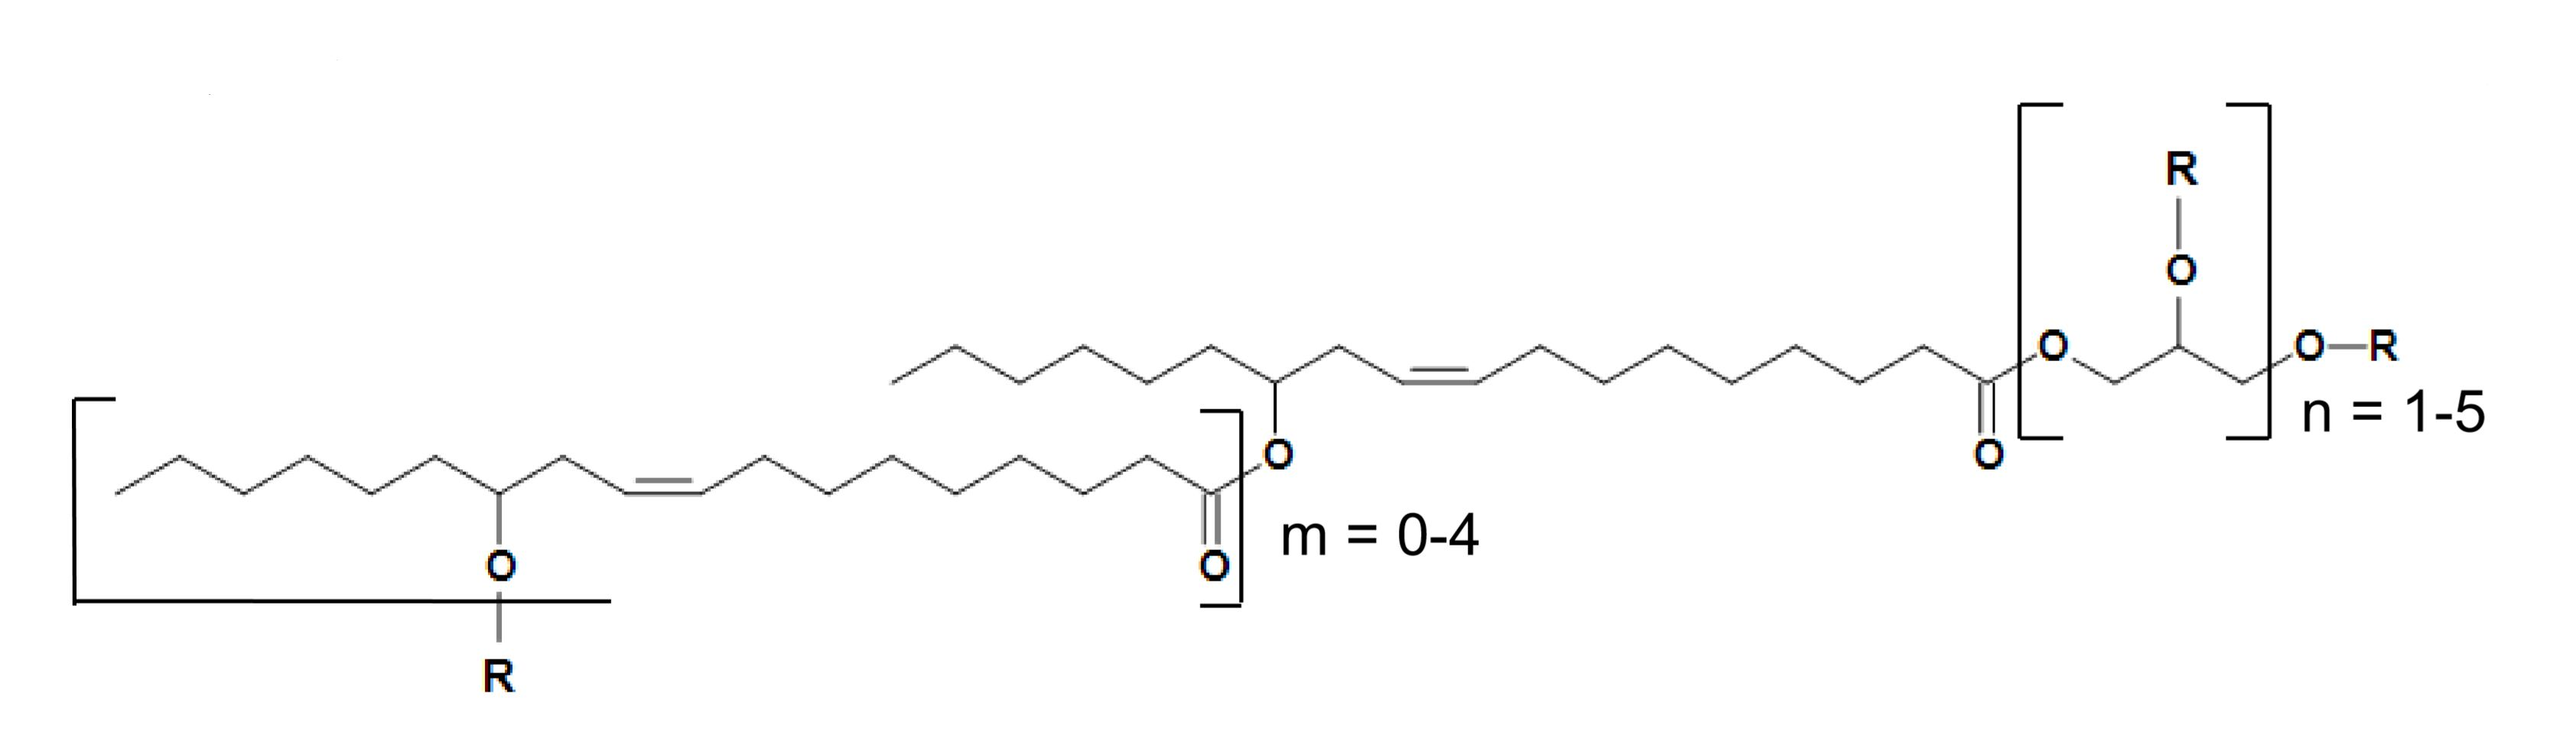
\includegraphics[width = 1\textwidth]{PGPR.JPG}
%\caption{Polyglycerin-polyricinoleat (PGPR)}
%\end{figure}
%\begin{figure}
%\centering
%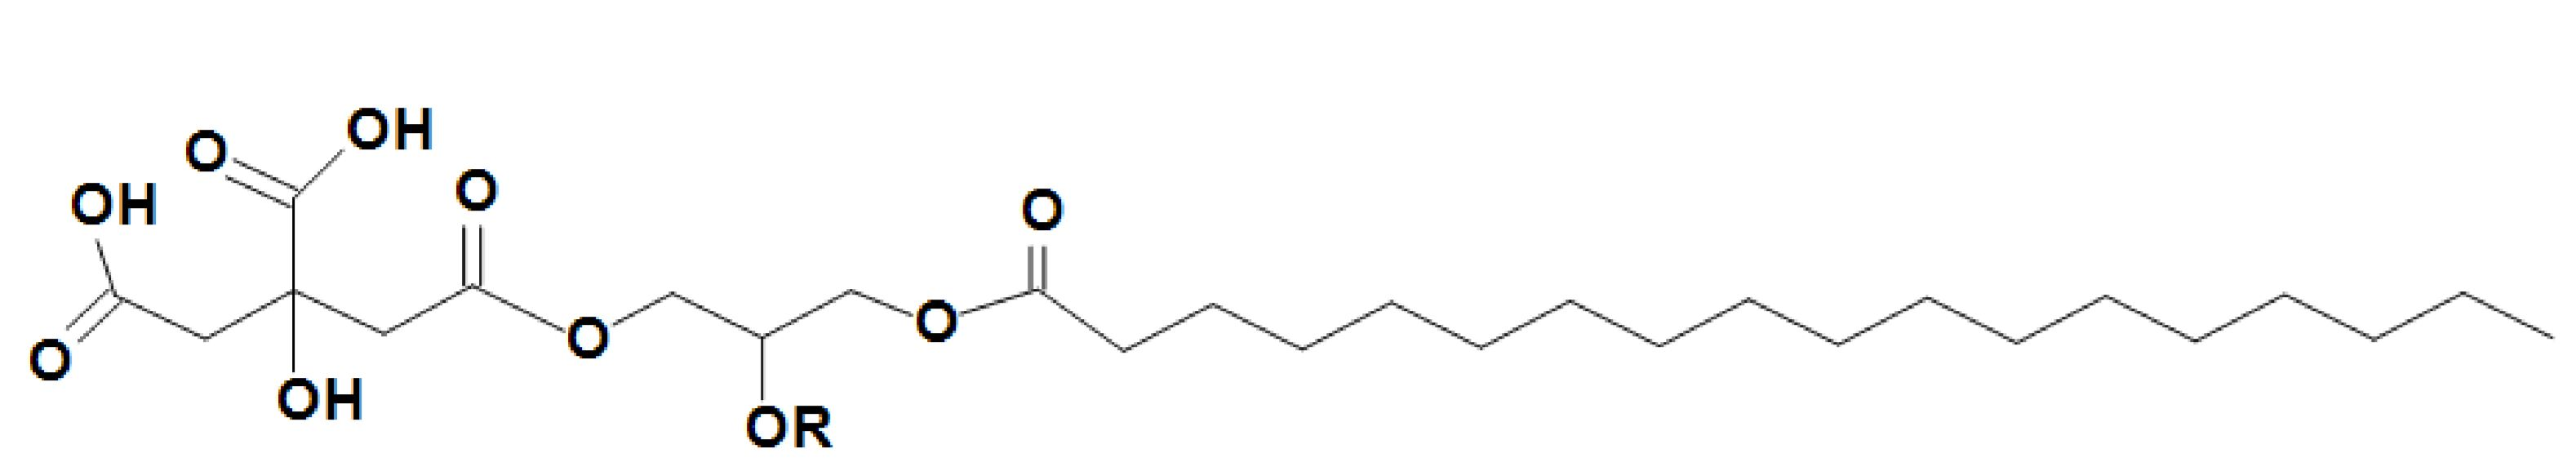
\includegraphics[width = 1\textwidth]{Zitronensaureester.JPG}
%\caption{Zitronensäureester}
%\end{figure}
%\end{frame}

\subsection{HLB-System}

\begin{frame}
\frametitle{Einteilung, das HLB-System}
\begin{block}{}
\begin{equation}
\text{HLB} = 20 \cdot \left(1-\frac{m_l}{m_{\text{ges}}}\right) = 20 \cdot \frac{m_h}{m_{\text{ges}}}
\end{equation}
$m_l$: Masse des lipophilen Teils \\
$m_h$: Masse des hydrophilen Kopfes
\end{block}


\pause
\begin{table}[H]
   \centering
   \begin{tabular}{|c|l|l|}
   \hline
   HLB-Bereich & Bezeichung &  Anwendung  \\
   \hline
   3 - 8 & W/O Emulgator & Saucen, Butter, Schokolade \\
   7 - 8 & & Feuchthaltemittel \\
   8 - 18 & O/W Emulgator & Vinaigrette, Mayonnaise! \\
   15- 18 & & Lösungsmittel \\
   \hline   
   \end{tabular}
\end{table}%
\begin{block}{}
Beispielwerte: Lecithin HLB = 4, PGPR HLB = 1.5
\end{block}


\end{frame}

\begin{frame}
\frametitle{Emulgatoren in kontinuierlicher Phase}
\begin{figure}[H]
\centering
\begin{subfigure}[c]{0.5\textwidth}
\centering
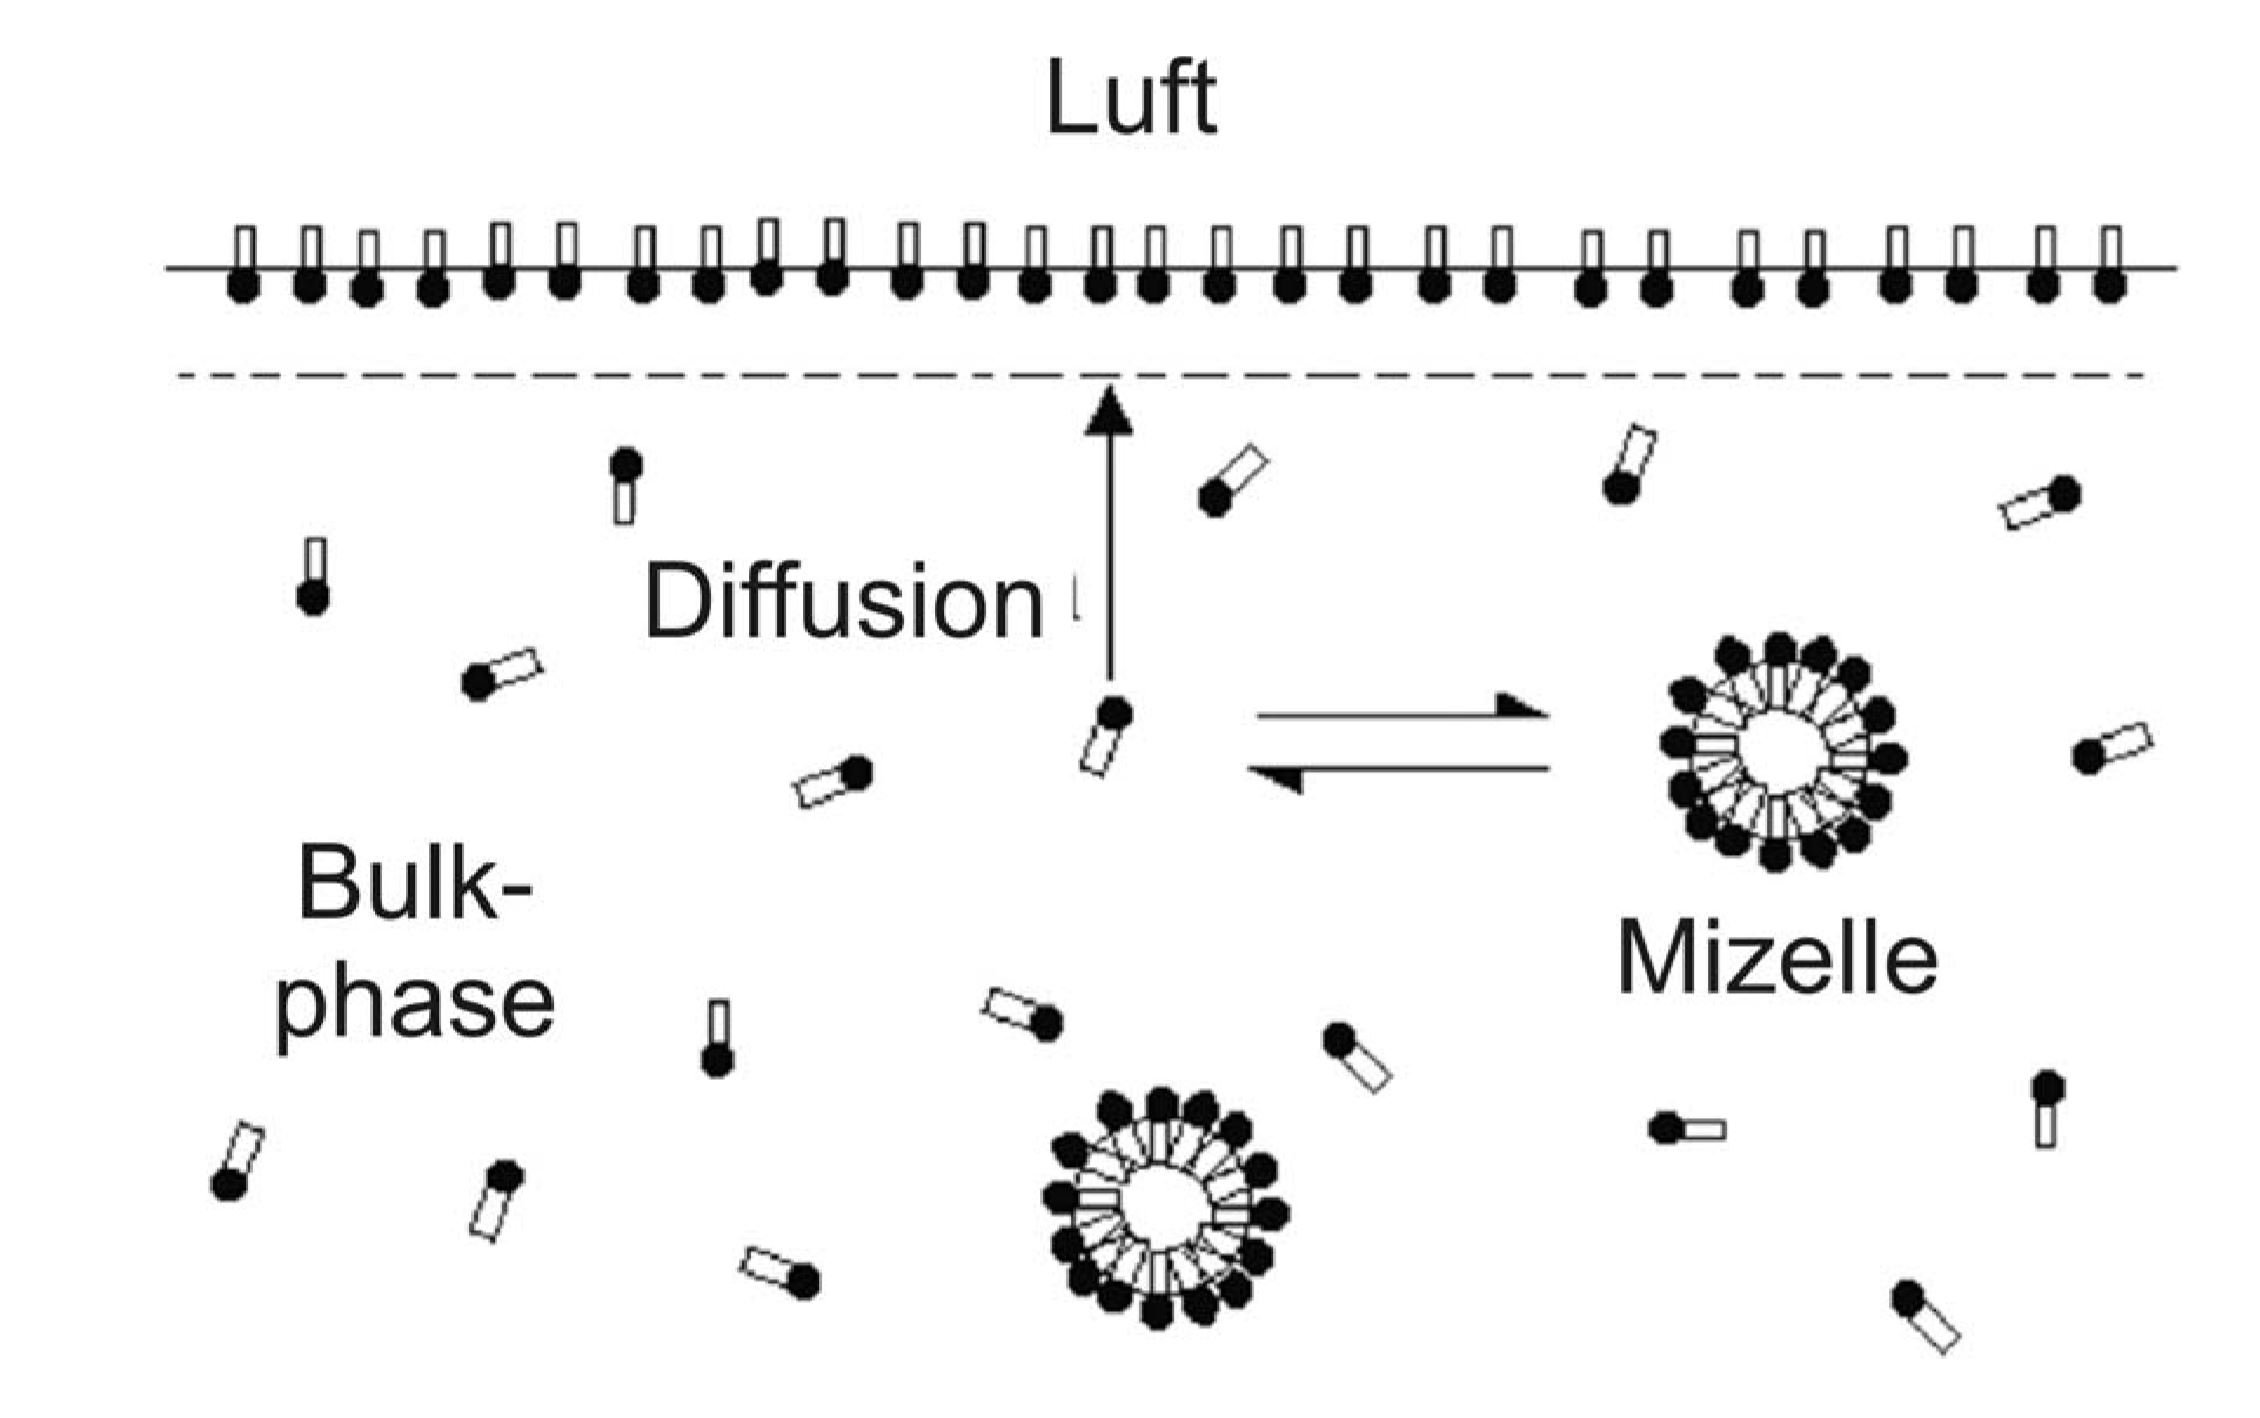
\includegraphics[width = 1\textwidth]{BulkPhase.JPG}
\end{subfigure}
\begin{subfigure}[c]{0.45\textwidth}
\centering
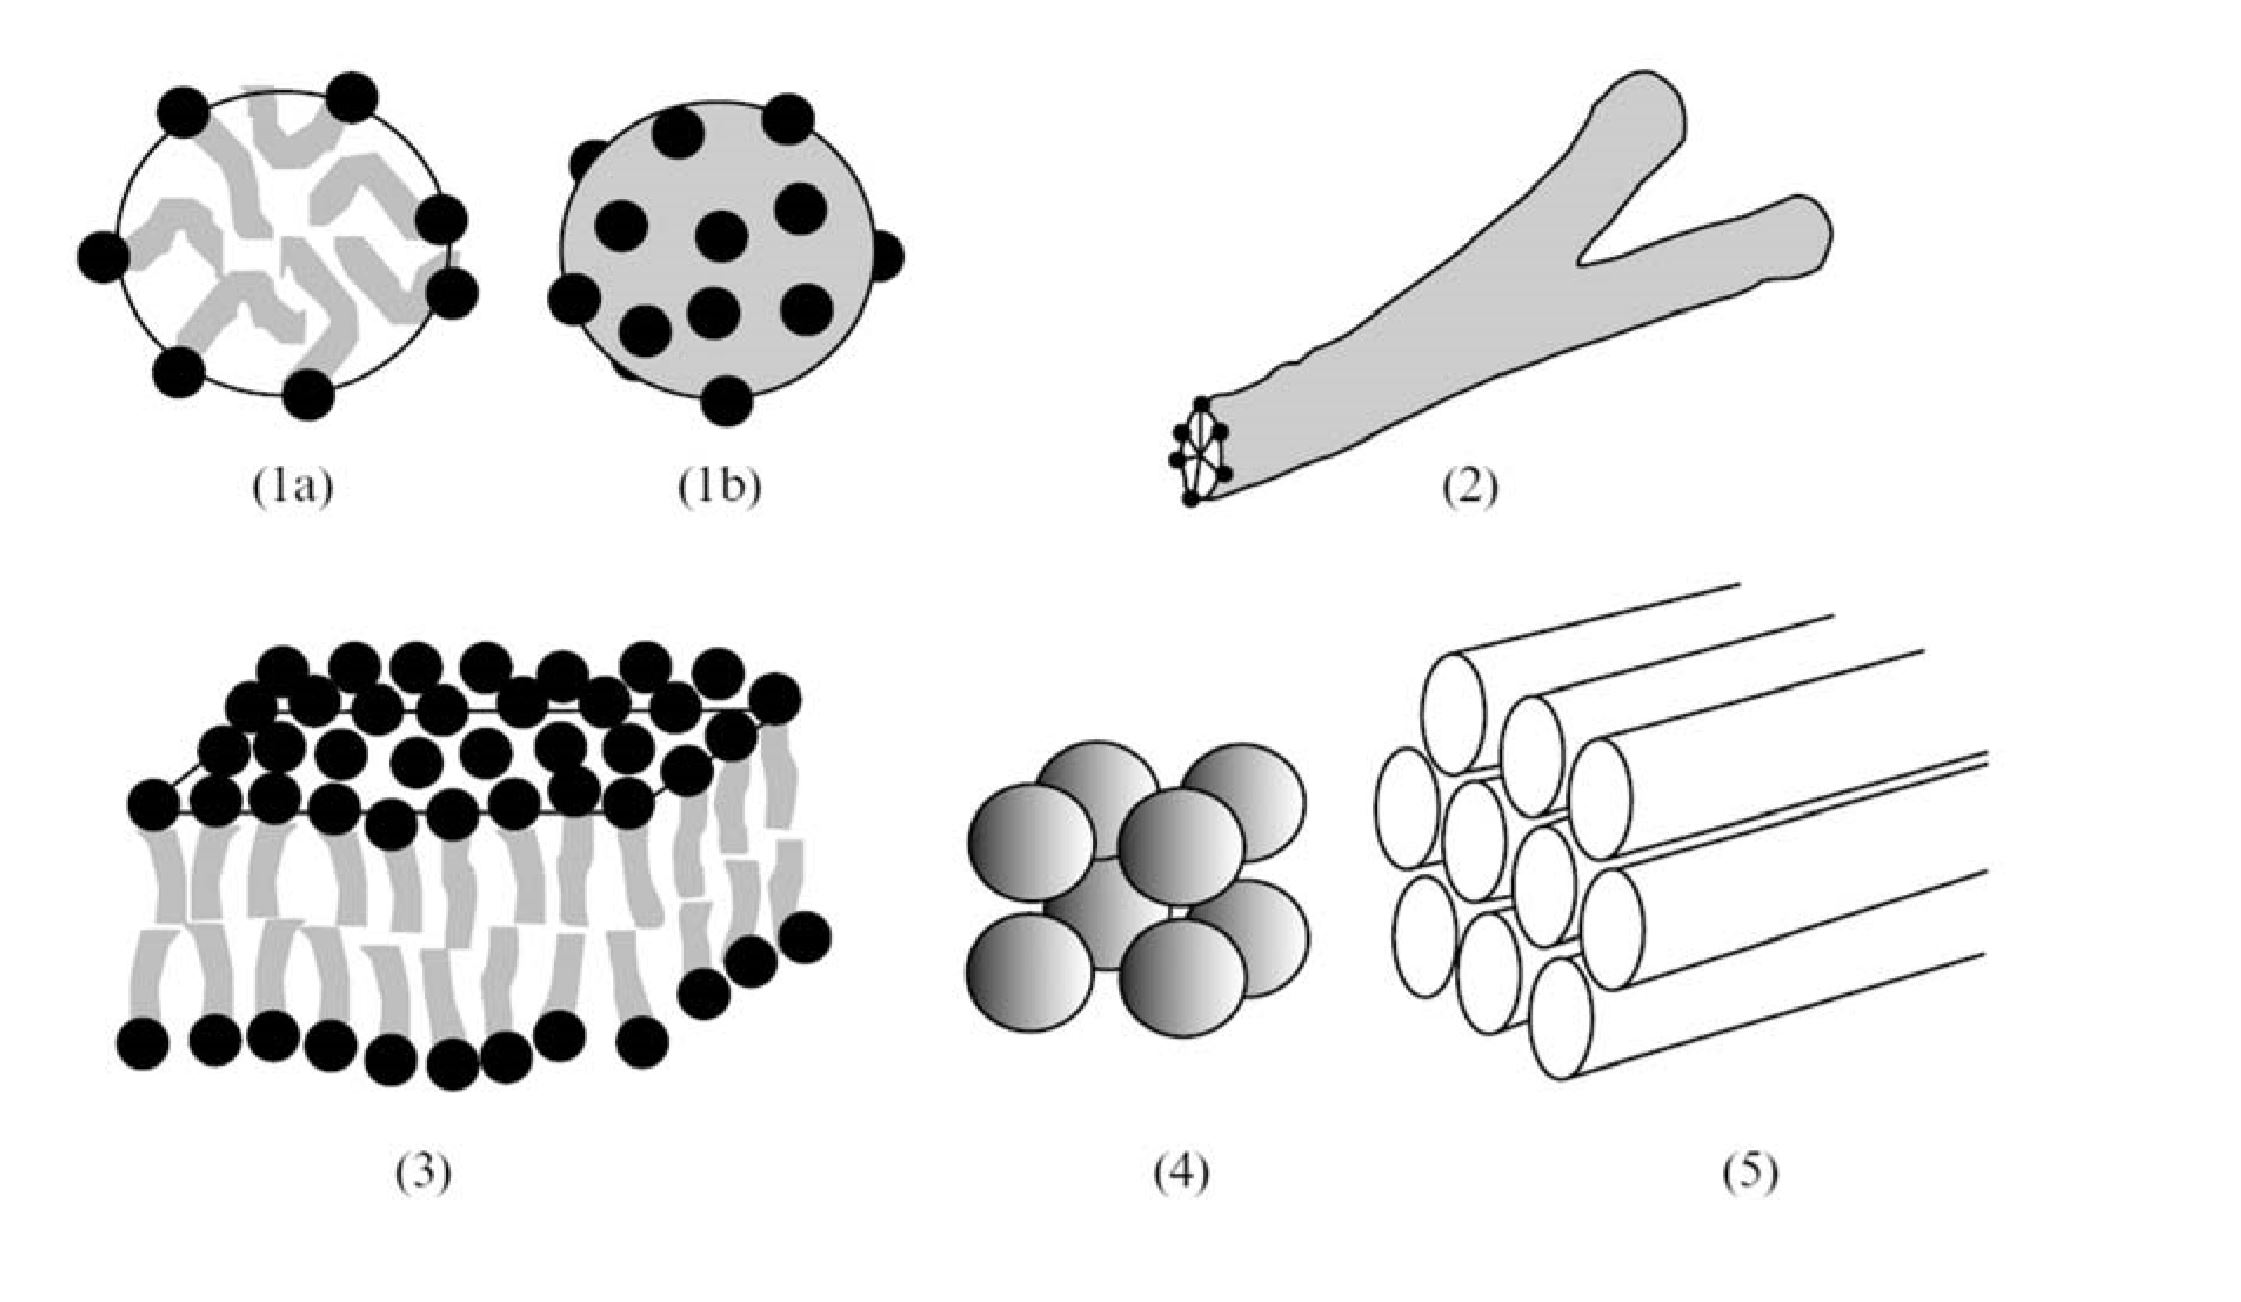
\includegraphics[width = 1\textwidth]{Mizellenarten.JPG}
\end{subfigure}
\end{figure}
\end{frame}

\subsection{Funktionsweise}

\begin{frame}
\frametitle{Emulgator in kontinuierlicher Phase}
\begin{figure}
\centering
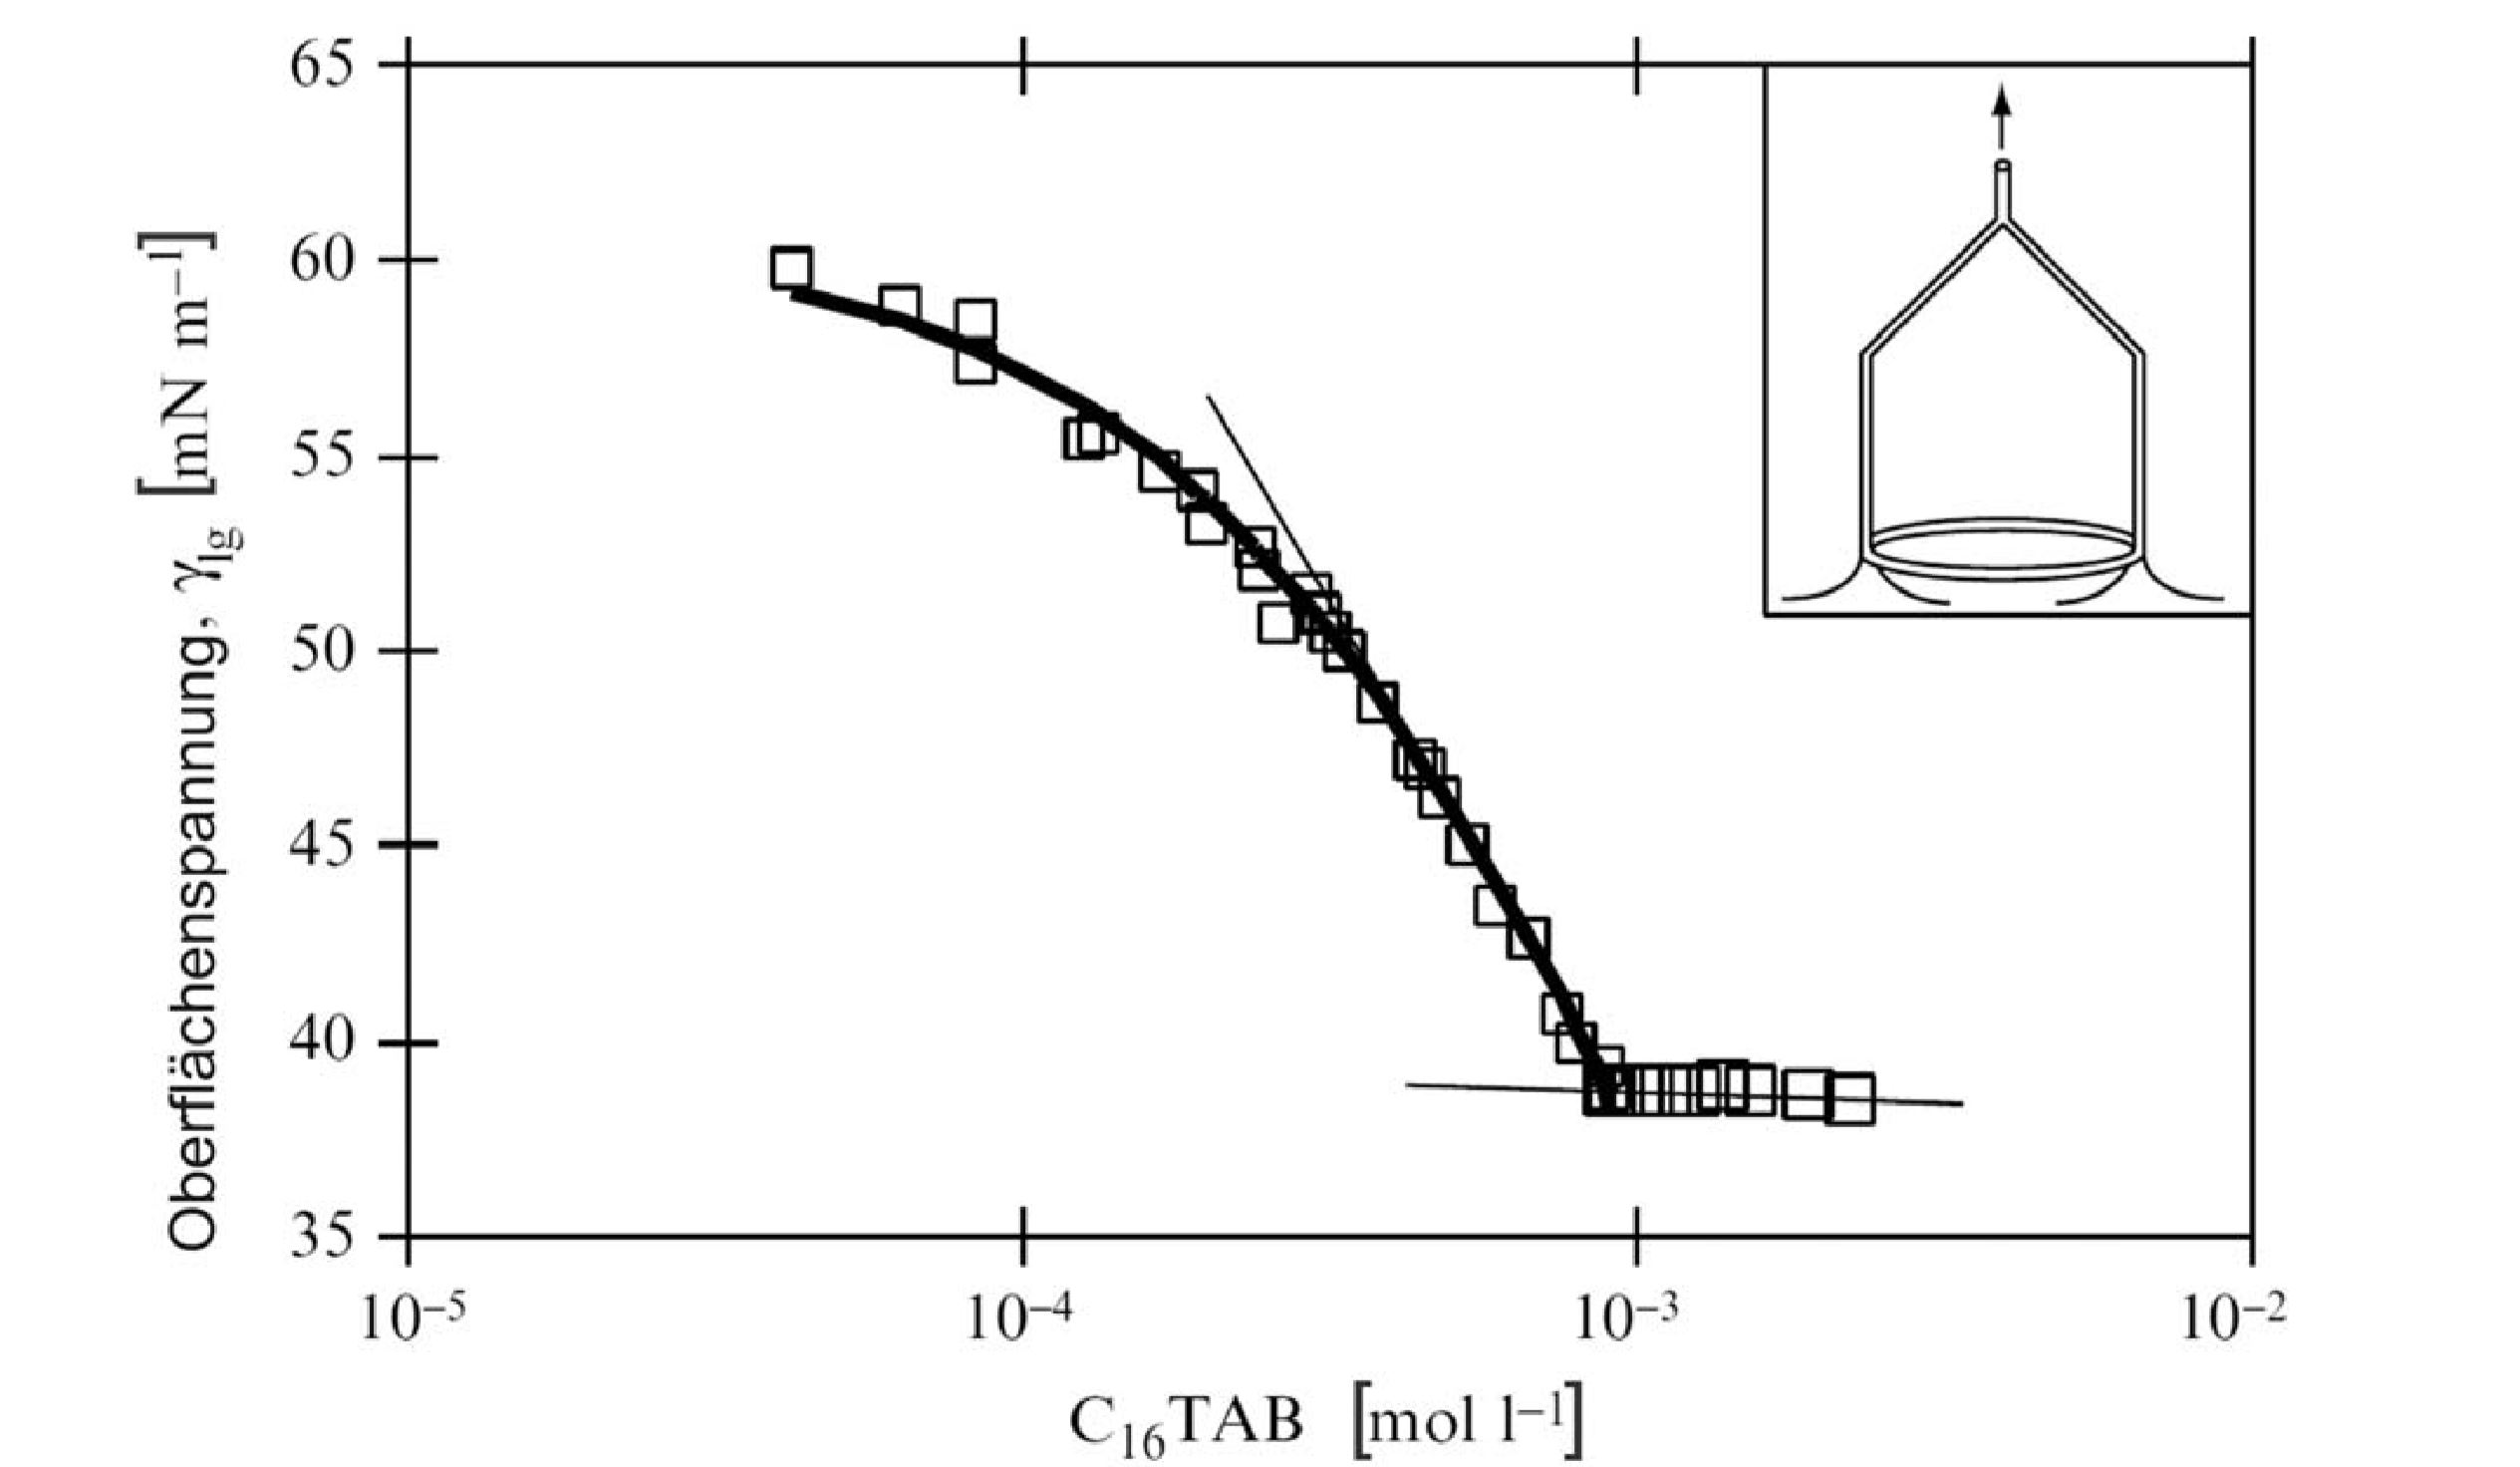
\includegraphics[width = 0.8\textwidth]{Oberflachenspannung.JPG}
\end{figure}
\end{frame}



\begin{frame}
\frametitle{Emulgator in Emulsion}
\begin{figure}
\centering
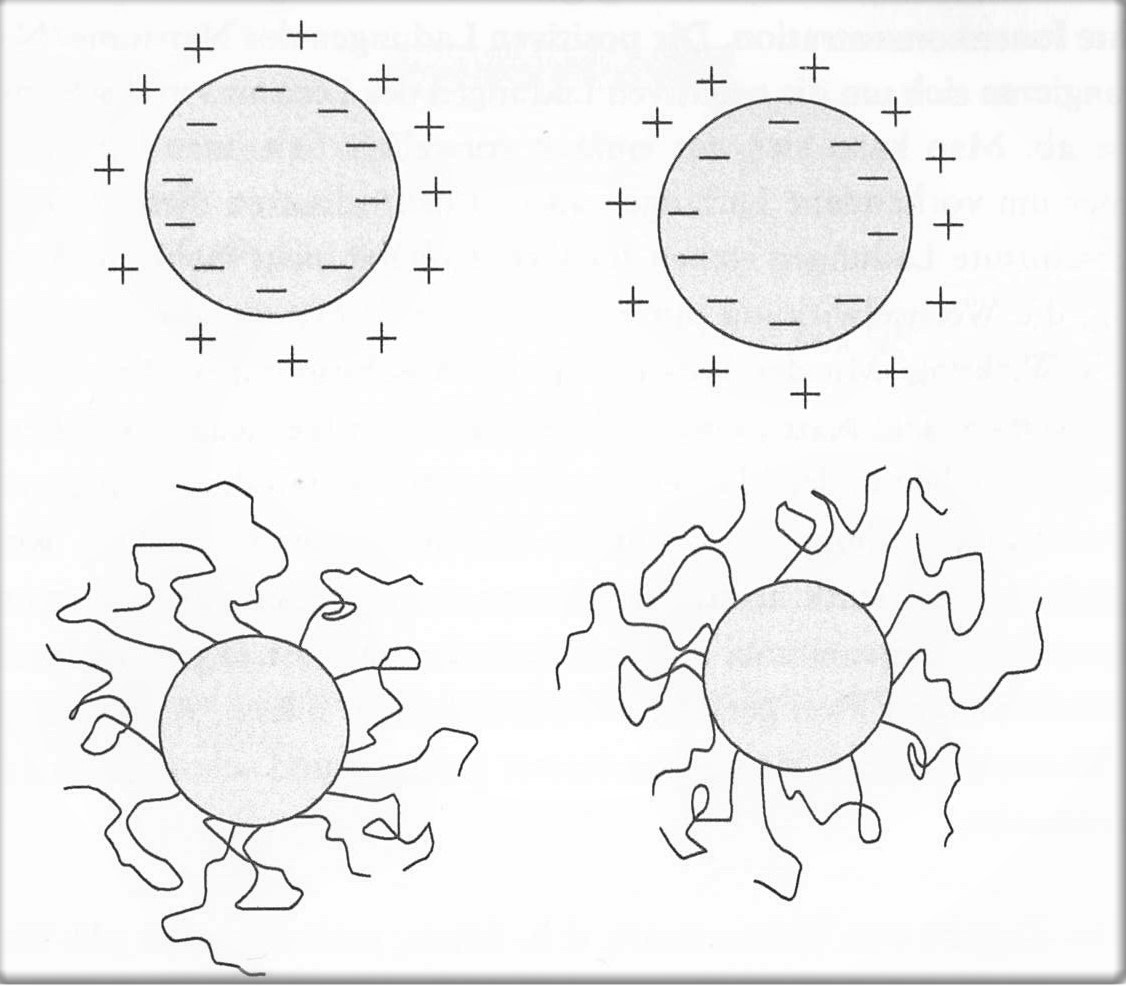
\includegraphics[width = 0.8\textwidth]{Wassertropfen.jpg}
\textcolor{white}{\cite{emulgierzentrifuge}}
\end{figure}
\end{frame}

\subsection{Anwendung: Mayonnaise}

\begin{frame}

\frametitle{Anwendung: Herstellen von Mayonnaise}

\begin{figure}
\centering
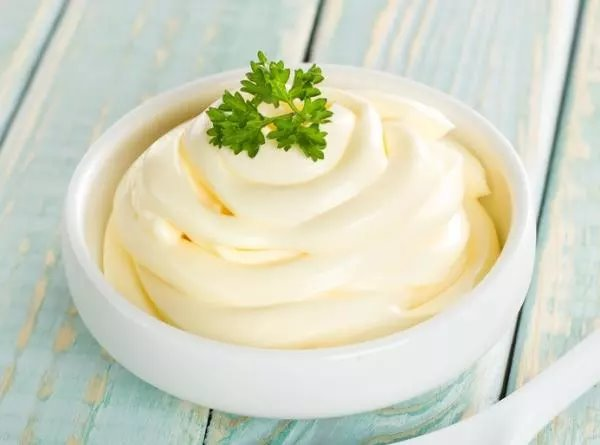
\includegraphics[width = 0.4\textwidth]{Mayonnaise.jpg}
\end{figure}
\pause
\begin{block}{\textcolor{white}{Tipps und Tricks}}
\begin{itemize}
\item Öl langsam zugeben
\item Säuren wie Zitronensaft zugeben
\item Am Ende Salzen
\item Eher von Hand rühren
\item Gleiche Temperatur
\end{itemize}
\end{block}

\end{frame}


\begin{frame}
\frametitle{Plumbers nightmare}
\begin{figure}[H]
\centering
\begin{subfigure}[c]{0.45\textwidth}
\centering
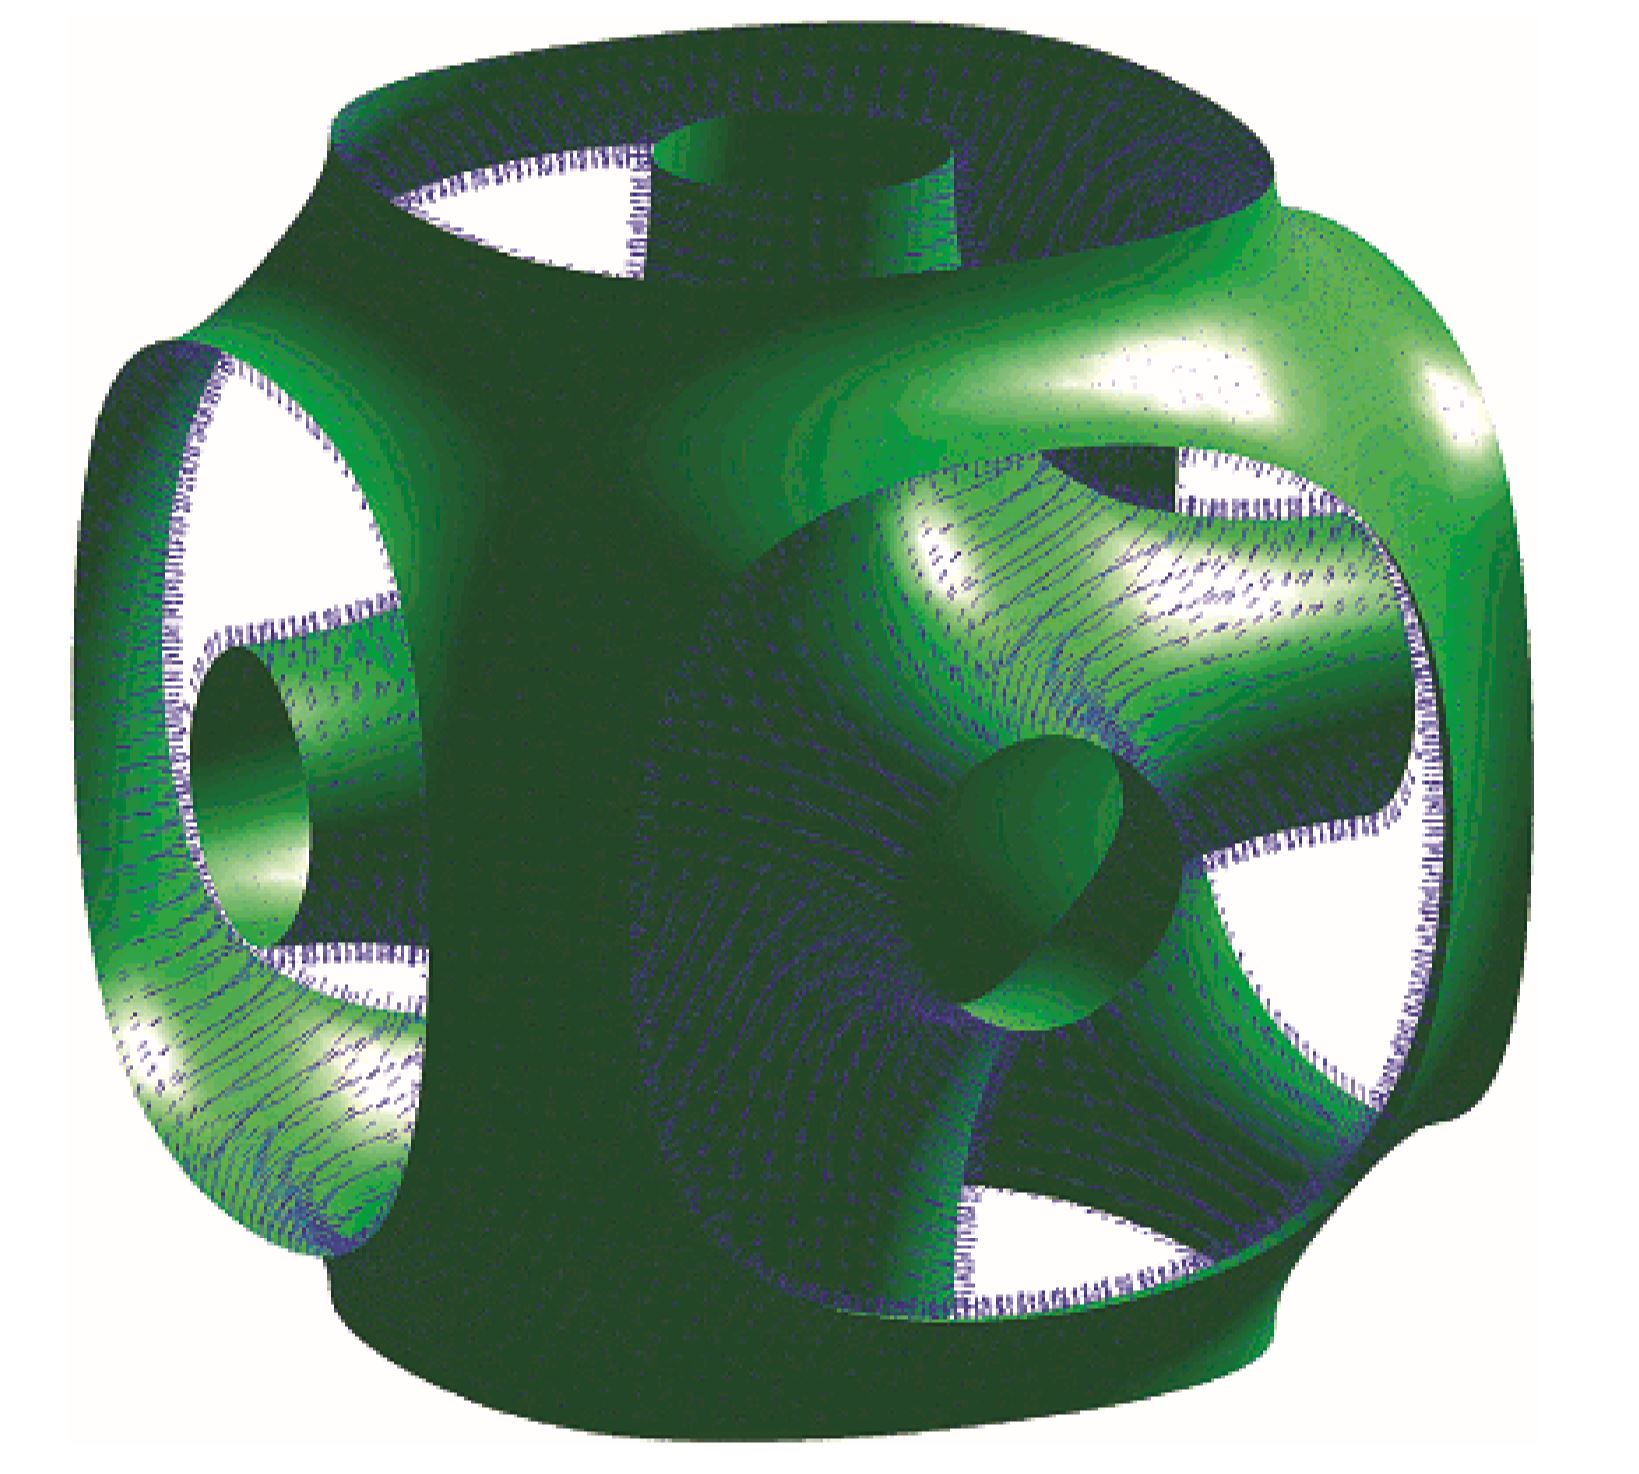
\includegraphics[width = 0.9\textwidth]{PlumbersNightmare1.JPG}
\end{subfigure}
\begin{subfigure}[c]{0.45\textwidth}
\centering
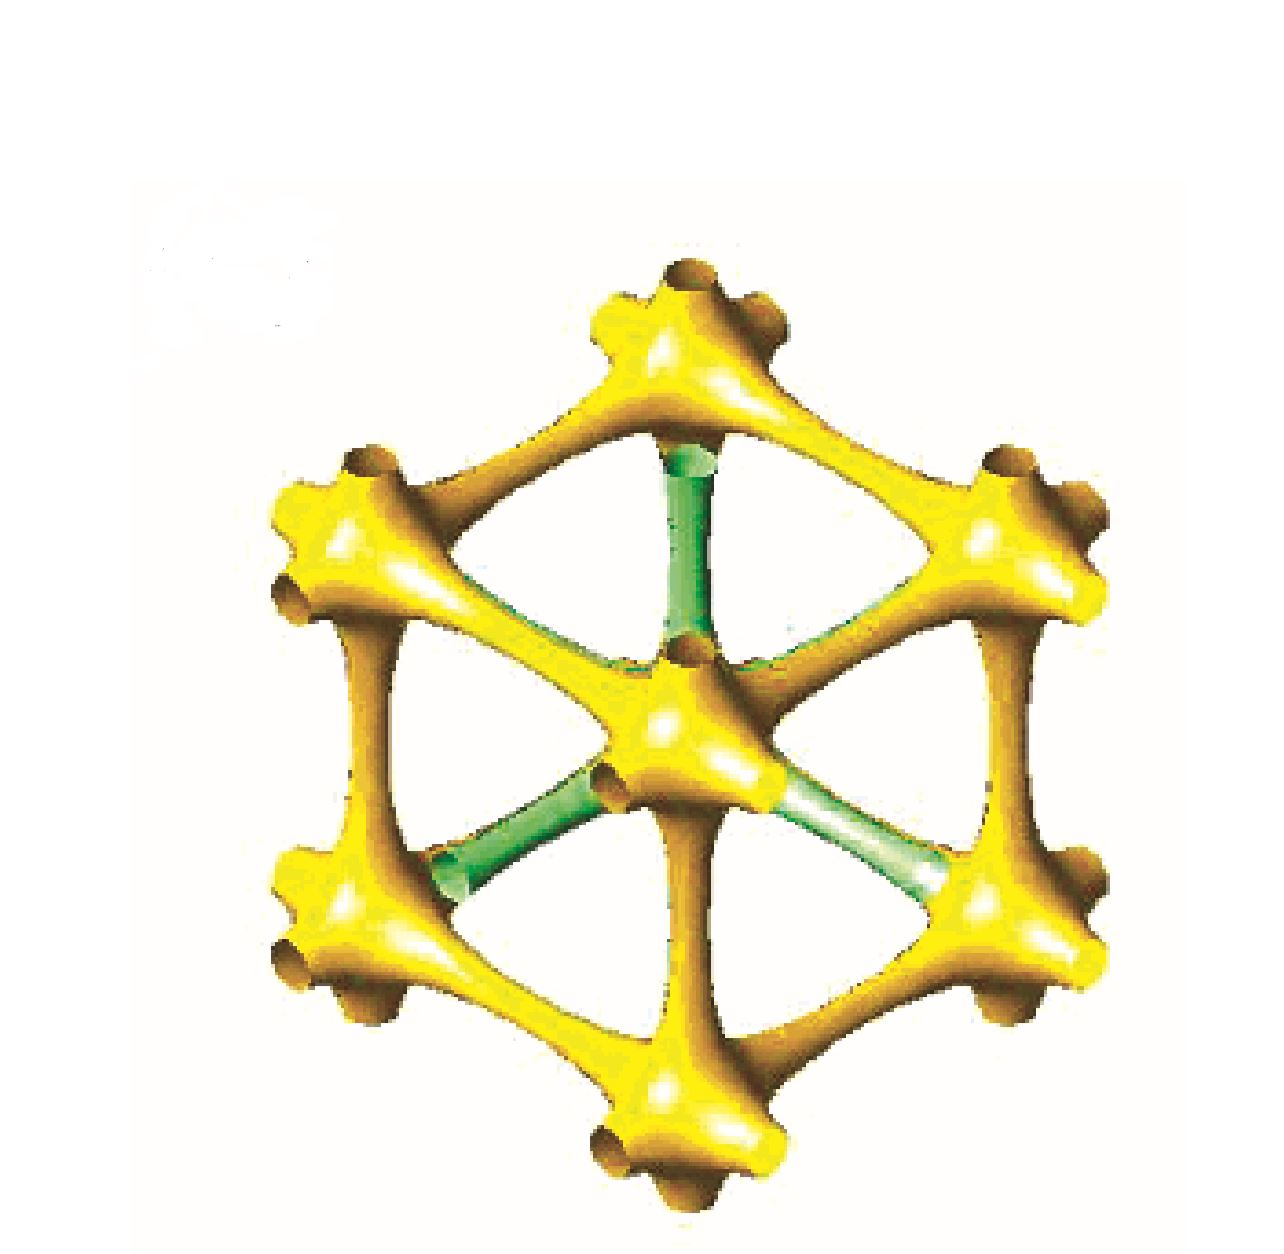
\includegraphics[width = 0.9\textwidth]{PlumbersNightmare2.JPG}
\end{subfigure}
\end{figure}

\end{frame}
\bibliographystyle{plain}
\bibliography{literature}
\addcontentsline{toc}{section}{Literature}

\begin{frame}
%Blinde Quellen
\cite{DocGrundlagen}
\cite{MolKueche}
\cite{Schokolade}
\cite{RatselKochkunst}
\end{frame}

\end{document}


